\documentclass[acmsmall,colorlinks, dvipsnames]{acmart}
%% colorlinks: option for package hyperref
%% dvipsnames: option for package xcolor

\usepackage{mystyle}
\usepackage{mymacros}
\usepackage{booktabs}
\usepackage{xtab}
\usepackage{physics}
\usepackage{amsmath}
\usepackage{tikz}
\usepackage{mathdots}
\usepackage{yhmath}
\usepackage{cancel}
\usepackage{color}
\usepackage{siunitx}
\usepackage{array}
\usepackage{multirow}
\usepackage{amssymb}
\usepackage{gensymb}
\usepackage{booktabs}
\usepackage{array}
\usetikzlibrary{fadings}
\usetikzlibrary{patterns}
\usetikzlibrary{shadows.blur}
\usetikzlibrary{shapes}
\usepackage{lineno}
\usepackage[normalem]{ulem}
\usepackage{tablefootnote}
\usepackage{colortbl}
\usepackage{makecell}
\usepackage[table]{xcolor}
\usepackage{tabularx}
\usepackage{threeparttable} %footnote for tables

\usepackage{url}
\def\UrlBreaks{\do\/\do-}
\usepackage{breakurl}
\usepackage{hyperref}
\usepackage{framed}

% Stretch whitespace a little bit to avoid overfull.
\emergencystretch=1em

\setcitestyle{numbers, comma}

%%Este comando eh usado para referenciar código PVS
% \newcommand{\pvscode}[1]{\texttt{#1}} 
\newcommand{\pvscode}[1]{\ensuremath{\mathit{#1}}} 
\newtheorem{axiom}{Axiom}

%\journal{Science of Computer Programming}

%%
%% These commands are for a JOURNAL article.
\acmJournal{TOSEM}

%% The following commands result in compilation errors if given empty arguments.
% \acmVolume{}
% \acmNumber{}
% \acmArticle{}
% \acmMonth{}



%\bibliographystyle{elsarticle-harv}
\bibliographystyle{model2-names}


\begin{document}
 
\selectlanguage{english}

%\begin{frontmatter}

%\linenumbers

\title{Analysis of Command and Control Strategy Through the Interaction of Software Components}

    % Authors
    
%Thiago
%Leopoldo
%Vander
%Sven
%Maxime
%Rohit

\author{Eduardo Lemos Rocha}
\affiliation{%
  \institution{University of Brasília}
  \streetaddress{Campus Universitário Darcy Ribeiro - Edifício CIC/EST, 70910-900}
  \city{Brasilia}
  \country{Brazil}}
\email{dudulr10@gmail.com}

\author{Vander Alves}
\affiliation{%
  \institution{University of Brasília}
  \streetaddress{Campus Universitário Darcy Ribeiro - Edifício CIC/EST, 70910-900}
  \city{Brasilia}
  \country{Brazil}}
\email{valves@unb.br}


%%
%% The abstract is a short summary of the work to be presented in the
%% article.
\begin{abstract}

A group of entities coordinating with each other to accomplish a common objective needs to cope with dynamic events to achieve success. By changing its current organization, the group can avoid unsatisfying results caused be the embedded dynamism related to the scenario. Although the presence of unexpected incidents is recognized in real world scenarios, the current state-of-art does not explore methodologies to increase the capability of handling new circumstances by changing the group's structure. To address this absence, we propose a computational model of a typed-parameterized extension of a channel system and its implementation in the Java Platform. The model is capable of dealing with context changes by providing communication among the group and coordination adjustments when necessary. To evaluate our solution, we conduct a simulation, which exposes the difference between the proposed model and the baseline approach, by a comparison between a series of established metrics.

\end{abstract}

%%
%% The code below is generated by the tool at http://dl.acm.org/ccs.cfm.
%%
\begin{CCSXML}
<ccs2012>
   <concept>
       <concept_id>10011007.10011074.10011092.10011096.10011097</concept_id>
       <concept_desc>Software and its engineering~Software product lines</concept_desc>
       <concept_significance>500</concept_significance>
       </concept>
   <concept>
       <concept_id>10011007.10011074.10011099.10011692</concept_id>
       <concept_desc>Software and its engineering~Formal software verification</concept_desc>
       <concept_significance>500</concept_significance>
       </concept>
 </ccs2012>
\end{CCSXML}

\ccsdesc[500]{Software and its engineering~Computing methodologies~Modeling and simulation~Simulation evaluation}
\ccsdesc[500]{Applied computing~Computers in other domains~Military}

\keywords{Command and Control, C2 Maneuver, Coordination, Channel System, Simulation}

%%
%% This command processes the author and affiliation and title
%% information and builds the first part of the formatted document.
\maketitle

\section{Introduction}
\label{sec:introduction}

% C2 + Example

\textit{Command and Control (C2)} is about focusing the efforts of a set of entities and resources towards the achievement of some task, objective, or goal~\citep{CC02}. The entities may represent individuals, organizations, systems, or a combination of these. Resources involve everything manipulated by the entities, including information exchange. Originally developed in military domain, C2 was based on the idea of a central command concentrating information and power over required elements to accomplish the mission~\citep{CC01}. Moreover, C2 applications include sensitive issues as nuclear weapon and research~\citep{C2-EX2}, national mass-vaccination campaigns~\citep{C2-EX1}, and the COVID-19 pandemic scenario, orchestrating different government and research organizations to find a mitigation or solution to the problem and providing responses to the society~\citep{C2-EX3, C2-EX4, C2-EX5}.

% C2 Agility -> Maneuver + Example + Relevance

\textit{C2 agility} is the entity's capability of dealing with context changes~\citep{france2014}. More complex scenarios caused by new circumstances require changing the collaboration approach among entities to deal with this dynamism in a suitable way. Hence, C2 agility needs to handle reorganization of the entities, i.e, changing the group's structure and functionalities. This branch of C2 agility, \textit{C2 Maneuver Agility}, is relevant due to the complexity of existing scenarios in C2. For instance, the sudden lack of entities or the increased risk of the scenario are some of the problems that characterize circumstance changes of C2 applied in the Civil Defense domain. Such scenario changes characterize context dynamism, which can occur in the mission, environment, or entity.

% Problem

Because a large variety of scenarios has embedded dynamism, it is important to be able to adapt the current organization of entities when is necessary. Otherwise, quality results may drop due to the new circumstances involved. In other words, the lack of C2 Maneuver Agility impacts the performance in these types of missions. Nevertheless, to the best of our knowledge, the current state-of-art does not explore methodologies or strategies to provide C2 Maneuver Agility, especially considering context changes~\cite{france2014, futureC2}.

% Solution

To provide C2 maneuver agility, we present a computational model that coordinates entities to handle context changes. Such model is a typed-parameterized extension of a channel system~\citep{modelcheckingBaier}. This extension, hereafter referred to as CS, defines the roles and responsibilities that are executed by the modelled entities. To cope with context changes, members can communicate and change their coordination structure thereby achieving C2 maneuver agility.

% Contributions

To asses the proposed computational model, we conduct a simulation. The simulation explores different scenarios with context changes. The results indicate that the entities have higher agility compared to baseline approach. We also identify challenging situations in achieving agility and discuss related tradeoffs. In summary, this work makes the following contributions:

\begin{itemize}
    \item We present a typed-paramaterized channel system modelling C2 system roles, their interactions, and dealing with context changes (Section~\ref{sec:channelSystem});
    \item We design and implement the proposed channel system and make it  publicly available\footnote{http://github.com/c2} (Section~\ref{sec:design});
    \item We perform a simulation-based study to empirically evaluate the proposed computational model in providing C2 maneuver agility, according to quality and quantity metrics (Section~\ref{sec:evaluation}). 
\end{itemize}

\section{Motivating Example}
\label{sec:motivation}

% Context and Explanation of the example
To provide intuition about the problem, we present an exemplification of a mission execution by entities in a military context. Figure \ref{fig:2TeamExecution} illustrates a reconnaissance mission with some tasks randomly distributed requiring different types of sensors. In this mission, a team comprising four Unmanned Aerial Vehicles (UAVs) is interacting in a network configuration with a central leader, which is responsible only for providing instructions to its subordinates, e.g, distributing tasks among members. These interactions and network topology configure a specific C2 approach, named as \textit{Coordinated}~\citep{france2014}, based on the centralized distribution of information, patterns of interaction, and decision rights. The leader, marked in blue, guides the other team members to complete the tasks, i.e., obtain aerial images of particular points in the field, represented by red crosses.

% Highlighting the problem
The mission involves some natural risks that may lead to change in the conditions of execution. In our example, one member of the team, marked in red, fell due to some environmental change, such as an intense storm, causing damage to its motors. The loss of one entity, as depicted in Figure \ref{fig:2Drop}, can potentially decrease the quality of execution, in case that the task of the fallen drone remain unattended. With this in mind, a new plan is required and must consider the new tasks that originally belong to the fallen drone. One possibility to avoid the problem is to change the current C2 approach, i.e., change the network configuration and leaders. Furthermore, if the team changes to an unsuitable C2 approach or is not even capable of changing its C2 approach, both cases represent a lack of C2 Maneuver Agility. The absence of a strategy to increase C2 Maneuver Agility can cause the system to compromise the number of completed tasks at the end of execution. 

\begin{figure}
\centering
\fbox{
\begin{minipage}{.45\textwidth}
  \centering
  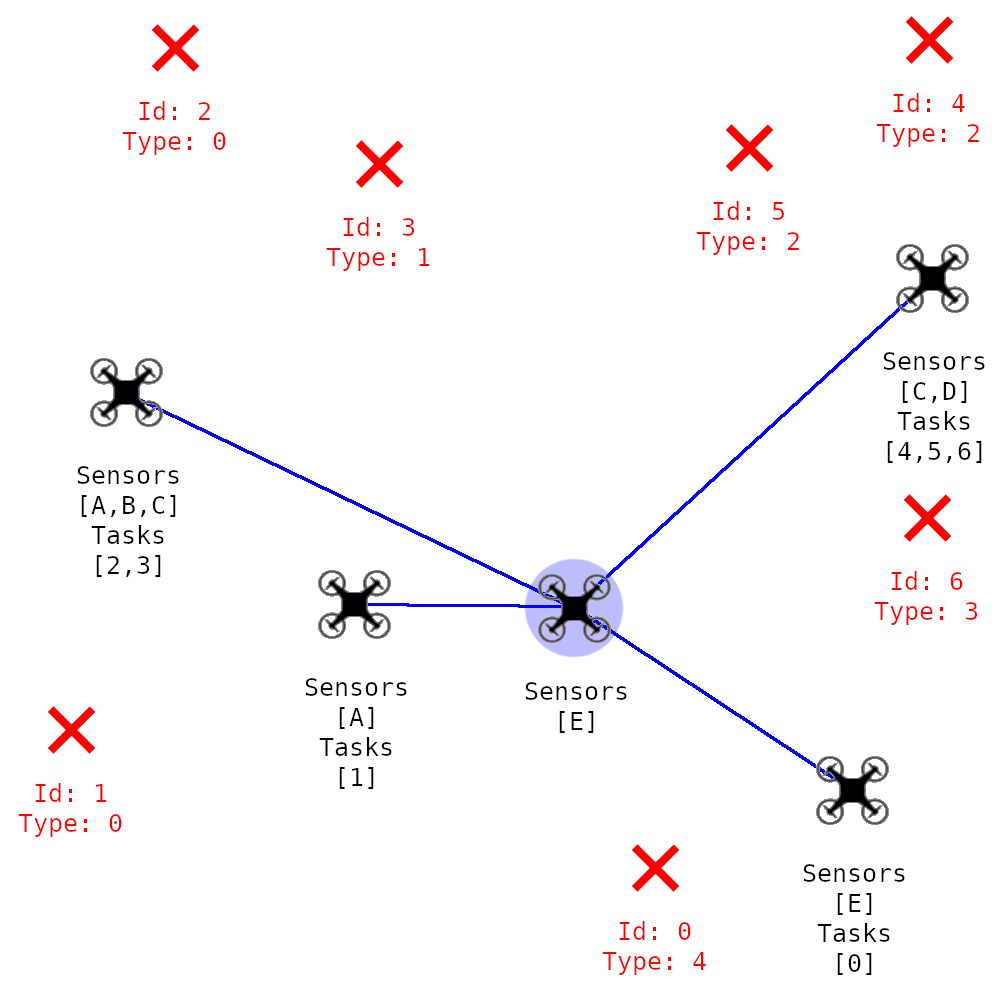
\includegraphics[width=0.95\linewidth]{figures/C2Drones1-V4.png}
  \captionof{figure}{Team of entities with the coordinator marked in blue}
  \label{fig:2TeamExecution}
\end{minipage}}%
\fbox{
\begin{minipage}{.45\textwidth}
  \centering
  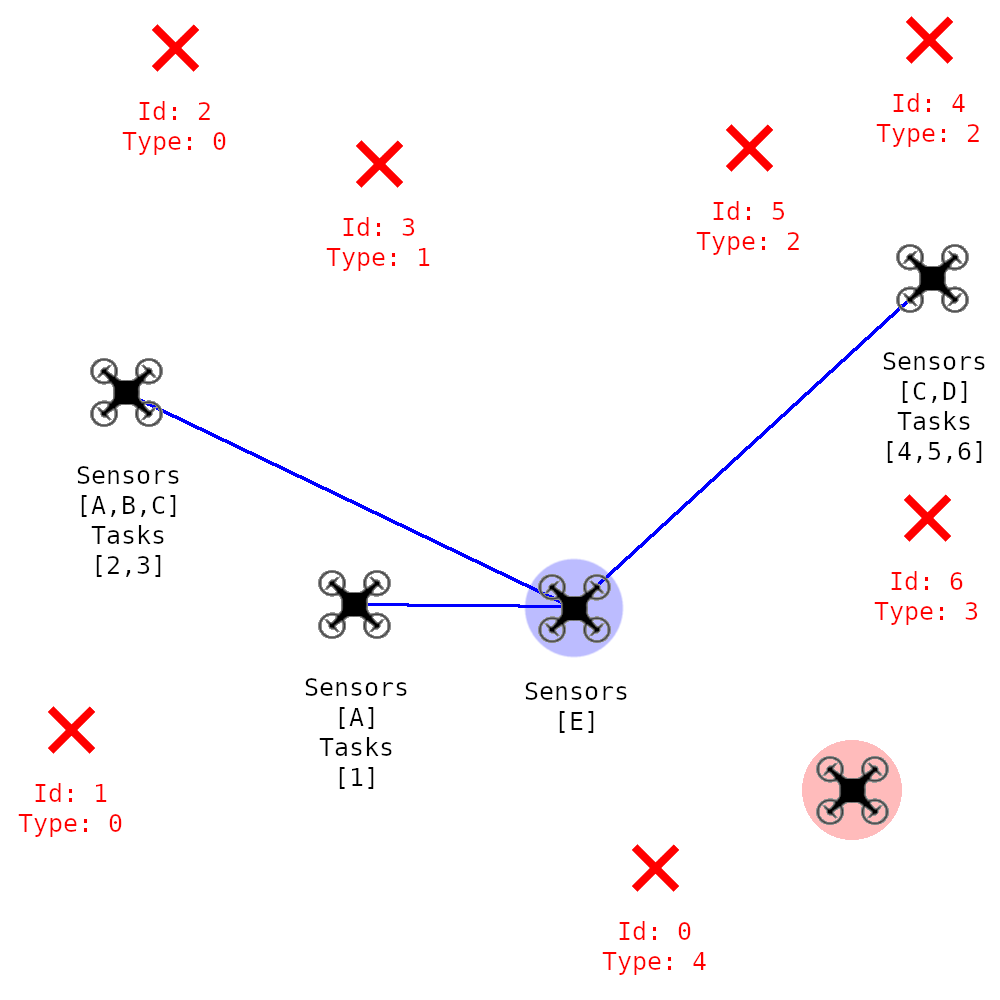
\includegraphics[width=0.95\linewidth]{figures/C2Drones2-V4.png}
  \captionof{figure}{Dynamic change with an UAV dropped marked in red}
  \label{fig:2Drop}
\end{minipage}}
\end{figure}

% Generalize the problem / Why is this not solved yet?
In general, some context changes, e.g., UAV failure, task addition, or sensor damage, must be considered during the mission planning. Indeed, no adaptation to the new context can impact quality results due to an incompatibility between entities and mission, or insufficient resources to complete the mission, or even the inability to meet minimum quality acceptance level. In other words, if there is limited C2 Maneuver Agility, the mission might be compromised.

Finally, Figure \ref{fig:3TeamExecutionAfterManuever} gives an example of a possible maneuvering strategy to maintain quality of execution. In this proposed example, immediately after the context change, the only member available for executing tasks type 4 is now offline. Moreover, the only member of the team capable of executing this new available task is the team's leader. Thus, after maneuvering to the \textit{Edge}~\citep{france2014} approach, the past leader can now participate in the execution of tasks, instead of only give orders to the team like in the previous strategy.

\begin{figure}[ht]
    \centering
    \fbox{
    \begin{minipage}{.45\textwidth}
  \centering
  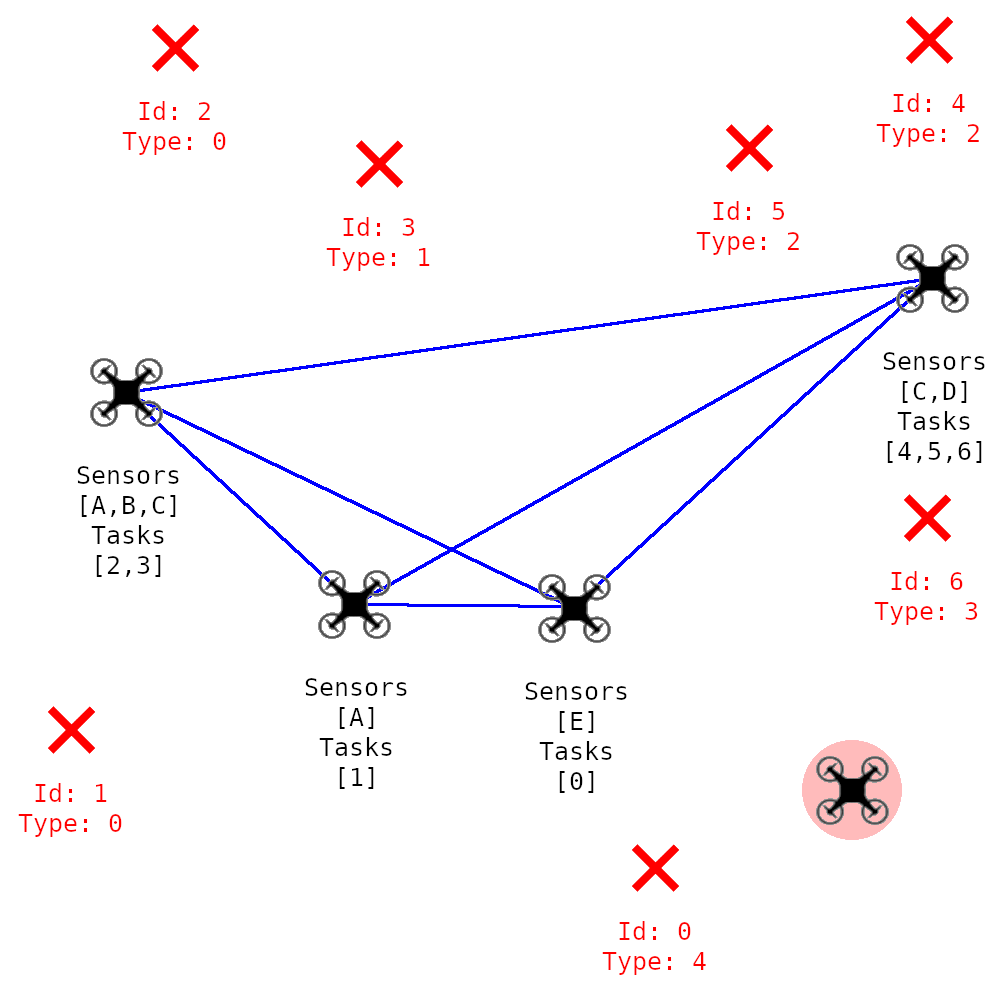
\includegraphics[width=0.95\linewidth]{figures/C2Drones3-V4.png}
  \captionof{figure}{Team executing tasks after changed C2 Approach}
  \label{fig:3TeamExecutionAfterManuever}
\end{minipage}}
\end{figure}
\section{Channel System}
\label{sec:channelSystem}

To justify and motivate the use of a CS, we need to establish our requirements. Recalling our motivation example (Section \ref{sec:motivation}), the team's members execute tasks in parallel and each member exchange information with the leader, changing its decisions based on the instructions its receives, i.e, which tasks are allocated for it. Moreover, dynamic events also changes its attitudes, e.g, sensor failure causes an information exchange with the leader, to update the task allocation process. Thus, the capability of coping with context changes eventually arising during a mission in a \textit{nondeterministic} way motivate the use of \textit{program graphs}~\cite{modelcheckingBaier}. Furthermore, the execution of parallel processes and the communication among members are requirements that prompt the use of \textit{channel systems}~\cite{modelcheckingBaier}.

A channel system is composed of a group of data-dependent processes communicating with each other via \textit{communication actions}~\cite{modelcheckingBaier}. With a program graph representing each process, transitions among states can be classified between conditional transitions or communication actions. Conditional transitions are important to avoid transitioning to states undesirably, according to boolean evaluations~\cite{modelcheckingBaier} defined during planning. The last type of transition works transmitting values through channels or receiving values from channels and assigning them to variables~\cite{modelcheckingBaier}. Additionally, channels can have a finite or infinite capacity of messages in a single channel, as well as a specified type of messages that can be stored in it. Finally, channel systems provide a notion of synchronization, whereas channels with a capacity different from zero function in a \textit{asynchronous} way and null capacity channels represent \textit{synchronous} communication~\cite{modelcheckingBaier}.

\begin{figure}[!ht]
    \centering
    \scalebox{.75}{

\tikzset{every picture/.style={line width=0.75pt}} %set default line width to 0.75pt        

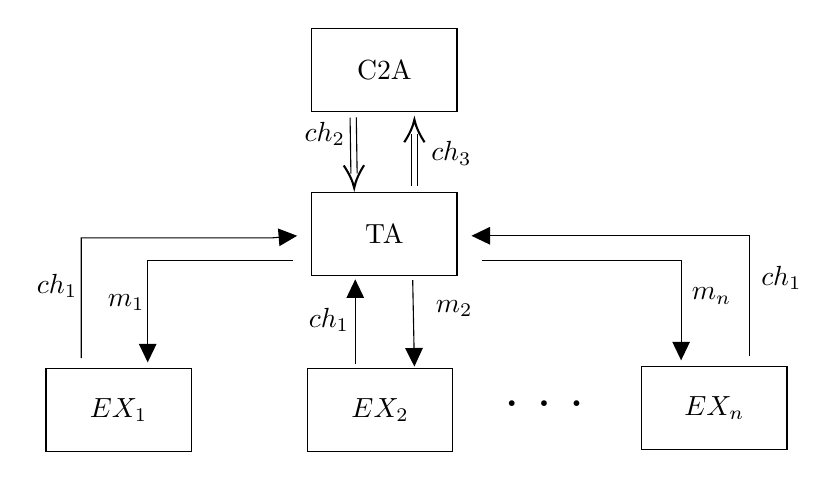
\begin{tikzpicture}[x=0.75pt,y=0.75pt,yscale=-1,xscale=1]
%uncomment if require: \path (0,225); %set diagram left start at 0, and has height of 225

%Shape: Rectangle [id:dp7793135649662085] 
\draw   (146,89) -- (216,89) -- (216,129) -- (146,129) -- cycle ;
%Shape: Rectangle [id:dp8388066725390221] 
\draw   (146,10) -- (216,10) -- (216,50) -- (146,50) -- cycle ;
%Shape: Rectangle [id:dp48691256180587716] 
\draw   (18,174) -- (88,174) -- (88,214) -- (18,214) -- cycle ;
%Straight Lines [id:da7136052167478543] 
\draw    (194.67,131.33) -- (195.44,170) ;
\draw [shift={(195.5,173)}, rotate = 268.85] [fill={rgb, 255:red, 0; green, 0; blue, 0 }  ][line width=0.08]  [draw opacity=0] (8.93,-4.29) -- (0,0) -- (8.93,4.29) -- cycle    ;
%Straight Lines [id:da1199439366931846] 
\draw    (35,169) -- (35,111) -- (127,111) -- (136.01,110.25) ;
\draw [shift={(139,110)}, rotate = 535.24] [fill={rgb, 255:red, 0; green, 0; blue, 0 }  ][line width=0.08]  [draw opacity=0] (8.93,-4.29) -- (0,0) -- (8.93,4.29) -- cycle    ;
%Shape: Rectangle [id:dp8070909053866772] 
\draw   (305,173) -- (375,173) -- (375,213) -- (305,213) -- cycle ;
%Shape: Rectangle [id:dp18131918632628874] 
\draw   (144,174) -- (214,174) -- (214,214) -- (144,214) -- cycle ;
%Straight Lines [id:da23459308482895536] 
\draw    (357,168) -- (357,110) -- (226,110) ;
\draw [shift={(223,110)}, rotate = 360] [fill={rgb, 255:red, 0; green, 0; blue, 0 }  ][line width=0.08]  [draw opacity=0] (8.93,-4.29) -- (0,0) -- (8.93,4.29) -- cycle    ;
%Straight Lines [id:da9340034396500284] 
\draw    (228,122) -- (324,122) -- (324,167) ;
\draw [shift={(324,170)}, rotate = 270] [fill={rgb, 255:red, 0; green, 0; blue, 0 }  ][line width=0.08]  [draw opacity=0] (8.93,-4.29) -- (0,0) -- (8.93,4.29) -- cycle    ;
%Straight Lines [id:da26523318096149495] 
\draw    (137,122) -- (67,122) -- (67,168) ;
\draw [shift={(67,171)}, rotate = 270] [fill={rgb, 255:red, 0; green, 0; blue, 0 }  ][line width=0.08]  [draw opacity=0] (8.93,-4.29) -- (0,0) -- (8.93,4.29) -- cycle    ;
%Straight Lines [id:da6224238934860249] 
\draw    (167,172) -- (167,134) ;
\draw [shift={(167,131)}, rotate = 450] [fill={rgb, 255:red, 0; green, 0; blue, 0 }  ][line width=0.08]  [draw opacity=0] (8.93,-4.29) -- (0,0) -- (8.93,4.29) -- cycle    ;
%Straight Lines [id:da30878293142018354] 
\draw    (167.5,52.98) -- (167.9,79.98)(164.5,53.02) -- (164.9,80.02) ;
\draw [shift={(166.5,87)}, rotate = 269.15999999999997] [color={rgb, 255:red, 0; green, 0; blue, 0 }  ][line width=0.75]    (10.93,-4.9) .. controls (6.95,-2.3) and (3.31,-0.67) .. (0,0) .. controls (3.31,0.67) and (6.95,2.3) .. (10.93,4.9)   ;
%Straight Lines [id:da1036410124215259] 
\draw    (197,61) -- (197,86)(194,61) -- (194,86) ;
\draw [shift={(195.5,54)}, rotate = 90] [color={rgb, 255:red, 0; green, 0; blue, 0 }  ][line width=0.75]    (10.93,-4.9) .. controls (6.95,-2.3) and (3.31,-0.67) .. (0,0) .. controls (3.31,0.67) and (6.95,2.3) .. (10.93,4.9)   ;

% Text Node
\draw (181,30) node   [align=left] {C2A};
% Text Node
\draw (181,109) node   [align=left] {TA};
% Text Node
\draw (53,194) node    {$EX_{1}$};
% Text Node
\draw (23.33,134.33) node    {$ch_{1}$};
% Text Node
\draw (214.67,145) node    {$m_{2}$};
% Text Node
\draw (340,193) node    {$EX_{n}$};
% Text Node
\draw (179,194) node    {$EX_{2}$};
% Text Node
\draw (258,191) node  [font=\Large] [align=left] {\textbf{. . .}};
% Text Node
\draw (338.67,139) node    {$m_{n}$};
% Text Node
\draw (56.67,142) node    {$m_{1}$};
% Text Node
\draw (154.33,150.33) node    {$ch_{1}$};
% Text Node
\draw (372.33,130.33) node    {$ch_{1}$};
% Text Node
\draw (152.33,60.83) node    {$ch_{2}$};
% Text Node
\draw (213.33,70.33) node    {$ch_{3}$};


\end{tikzpicture}}
    \caption{Proposed Channel System}
    \label{fig:CS}
\end{figure}

Figure \ref{fig:CS} illustrates our channel system. The proposed channel system describes our coordination strategy. We decided to model our coordination using separate roles, mainly due to its nature of modulatizing functional aspects~\cite{roleOrientedModeling}. Also, roles are used to define positions within an organization, encapsulating certain tasks, responsibilities, and goals that an owner of a role has to fulfil~\cite{roleOrientedModeling}. Thus, each member of the team can posses a program graph that describes a distinct role, and more than one role can coexist in the same entity. Also, during maneuvering between different C2 approaches~\cite{france2014}, roles assignment can be changed, providing more possibilities to the team during the mission.

To modularize roles, we divided the coordination aspect among two different roles:

\begin{itemize}
    \item Task Allocator (TA): responsible for distributing tasks throughout the team, based on team members attributes, such as fuel and sensors onboard. Moreover, this role reports results provided by executors to the C2 approach selector role;
    \item C2 Approach Selector (C2S): responsible for detecting the need of changing the C2 approach, due to some drop in performance reported by task allocator. Additionally, it communicates to task allocator if a maneuver will occur.  
\end{itemize}

Furthermore, each member executes its set of roles encapsulated in it. For instance, as depicted in Figure \ref{fig:CS}, each member playing the executor (EX) role communicates with the leader, i.e, member who plays the role TA, using channel \textit{$ch_1$} in a asynchronous manner. Similarly, the leader provides tasks to each executor member using channel \textit{$m_i$} whereas $i$ is the executor's index. Finally, the C2S role and TA role exchange information using synchronized channels \textit{$ch_2$} and \textit{$ch_3$} to asses performance and check if a maneuver is crucial to maintain quality of execution during the mission. These latter channels use synchronized communication because the TA role provides performance information using channel \textit{$ch_3$} and waits for the C2S's response to know if a maneuver might happen. Until this feedback information approaches the channel \textit{$ch_2$}, the TA role stops allocating tasks to the remaining members. However, members that execute tasks, i.e, play the EX role, and allocate tasks, i.e, play the TA role, don't need to wait for any response and can continue executing tasks or allocating tasks, justifying the asynchronous communication between these roles.

\begin{figure}[!ht]
    \centering
    \scalebox{.65}{

\tikzset{every picture/.style={line width=0.75pt}} %set default line width to 0.75pt        

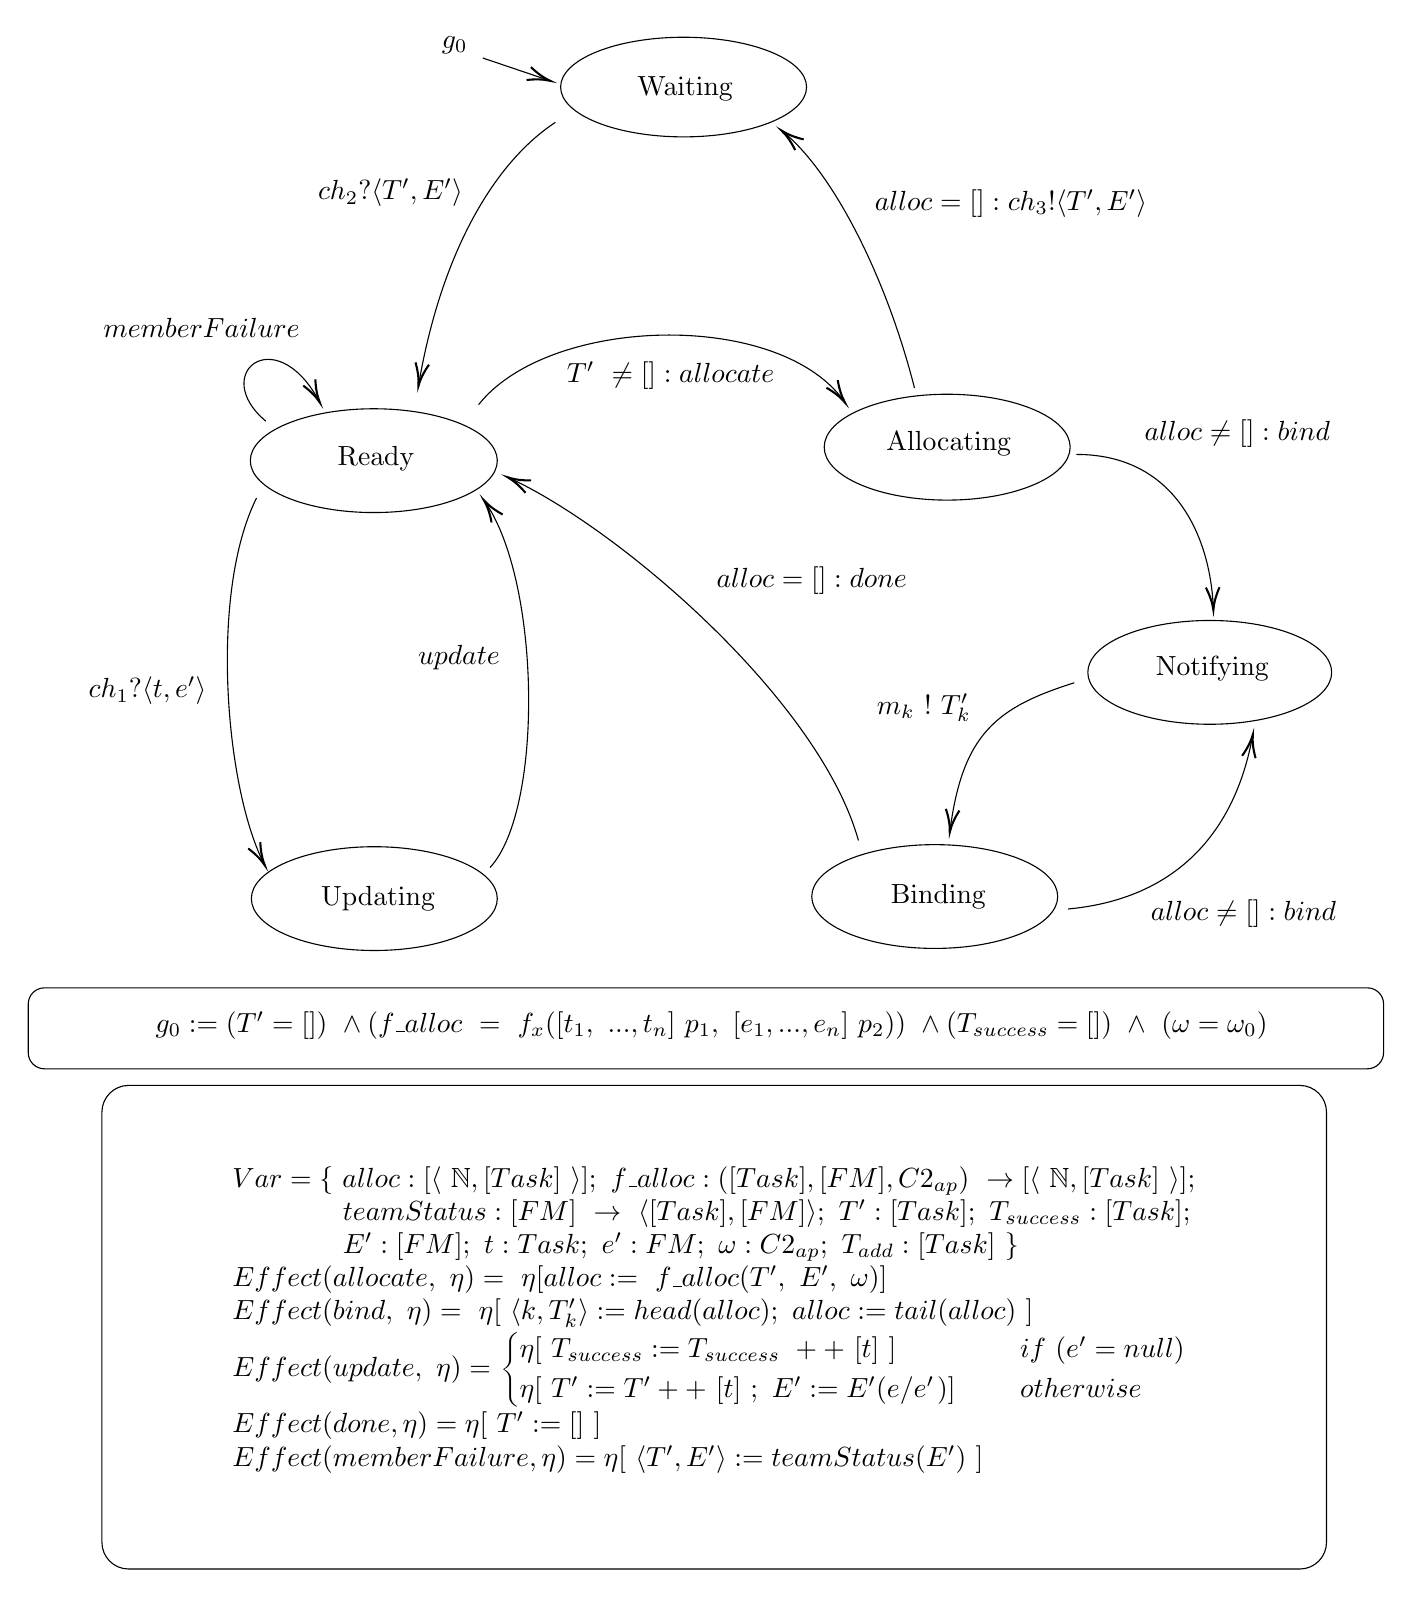
\begin{tikzpicture}[x=0.75pt,y=0.75pt,yscale=-1,xscale=1]
%uncomment if require: \path (0,754); %set diagram left start at 0, and has height of 754

%Curve Lines [id:da9480858267519683] 
\draw    (230.5,181) .. controls (264.16,138.43) and (373.78,135.06) .. (406.05,178.66) ;
\draw [shift={(407,180)}, rotate = 235.44] [color={rgb, 255:red, 0; green, 0; blue, 0 }  ][line width=0.75]    (10.93,-3.29) .. controls (6.95,-1.4) and (3.31,-0.3) .. (0,0) .. controls (3.31,0.3) and (6.95,1.4) .. (10.93,3.29)   ;
%Shape: Ellipse [id:dp6594609066072359] 
\draw   (120.5,208) .. controls (120.5,194.19) and (147.14,183) .. (180,183) .. controls (212.86,183) and (239.5,194.19) .. (239.5,208) .. controls (239.5,221.81) and (212.86,233) .. (180,233) .. controls (147.14,233) and (120.5,221.81) .. (120.5,208) -- cycle ;
%Shape: Ellipse [id:dp873836537729809] 
\draw   (397,201.5) .. controls (397,187.42) and (423.53,176) .. (456.25,176) .. controls (488.97,176) and (515.5,187.42) .. (515.5,201.5) .. controls (515.5,215.58) and (488.97,227) .. (456.25,227) .. controls (423.53,227) and (397,215.58) .. (397,201.5) -- cycle ;
%Curve Lines [id:da14662580418826565] 
\draw    (514.5,424) .. controls (567.96,419.05) and (594.96,385.68) .. (603.25,341.35) ;
\draw [shift={(603.5,340)}, rotate = 460.08] [color={rgb, 255:red, 0; green, 0; blue, 0 }  ][line width=0.75]    (10.93,-3.29) .. controls (6.95,-1.4) and (3.31,-0.3) .. (0,0) .. controls (3.31,0.3) and (6.95,1.4) .. (10.93,3.29)   ;
%Straight Lines [id:da37650774099478246] 
\draw    (232.5,14) -- (263.11,24.36) ;
\draw [shift={(265,25)}, rotate = 198.7] [color={rgb, 255:red, 0; green, 0; blue, 0 }  ][line width=0.75]    (10.93,-3.29) .. controls (6.95,-1.4) and (3.31,-0.3) .. (0,0) .. controls (3.31,0.3) and (6.95,1.4) .. (10.93,3.29)   ;
%Shape: Ellipse [id:dp8139093405894636] 
\draw   (121,419) .. controls (121,405.19) and (147.53,394) .. (180.25,394) .. controls (212.97,394) and (239.5,405.19) .. (239.5,419) .. controls (239.5,432.81) and (212.97,444) .. (180.25,444) .. controls (147.53,444) and (121,432.81) .. (121,419) -- cycle ;
%Shape: Ellipse [id:dp08678607998247811] 
\draw   (391,418) .. controls (391,404.19) and (417.53,393) .. (450.25,393) .. controls (482.97,393) and (509.5,404.19) .. (509.5,418) .. controls (509.5,431.81) and (482.97,443) .. (450.25,443) .. controls (417.53,443) and (391,431.81) .. (391,418) -- cycle ;
%Shape: Ellipse [id:dp07482494496489733] 
\draw   (270,28) .. controls (270,14.75) and (296.53,4) .. (329.25,4) .. controls (361.97,4) and (388.5,14.75) .. (388.5,28) .. controls (388.5,41.25) and (361.97,52) .. (329.25,52) .. controls (296.53,52) and (270,41.25) .. (270,28) -- cycle ;
%Curve Lines [id:da6759956440889884] 
\draw    (123.5,226) .. controls (100.84,271.31) and (108.27,364.16) .. (126.65,401.34) ;
\draw [shift={(127.5,403)}, rotate = 242.18] [color={rgb, 255:red, 0; green, 0; blue, 0 }  ][line width=0.75]    (10.93,-3.29) .. controls (6.95,-1.4) and (3.31,-0.3) .. (0,0) .. controls (3.31,0.3) and (6.95,1.4) .. (10.93,3.29)   ;
%Curve Lines [id:da9572857730465772] 
\draw    (234.22,228.76) .. controls (260.54,268.31) and (261.61,376.42) .. (236,404) ;
\draw [shift={(233,227)}, rotate = 54.11] [color={rgb, 255:red, 0; green, 0; blue, 0 }  ][line width=0.75]    (10.93,-3.29) .. controls (6.95,-1.4) and (3.31,-0.3) .. (0,0) .. controls (3.31,0.3) and (6.95,1.4) .. (10.93,3.29)   ;
%Curve Lines [id:da9385545433271328] 
\draw    (517.5,315) .. controls (479.88,326.88) and (463.82,339.74) .. (457.68,385.6) ;
\draw [shift={(457.5,387)}, rotate = 277.28] [color={rgb, 255:red, 0; green, 0; blue, 0 }  ][line width=0.75]    (10.93,-3.29) .. controls (6.95,-1.4) and (3.31,-0.3) .. (0,0) .. controls (3.31,0.3) and (6.95,1.4) .. (10.93,3.29)   ;
%Curve Lines [id:da13526468384837043] 
\draw    (440.5,173) .. controls (426.78,119.1) and (401.54,70) .. (377.94,50.18) ;
\draw [shift={(376.5,49)}, rotate = 398.37] [color={rgb, 255:red, 0; green, 0; blue, 0 }  ][line width=0.75]    (10.93,-3.29) .. controls (6.95,-1.4) and (3.31,-0.3) .. (0,0) .. controls (3.31,0.3) and (6.95,1.4) .. (10.93,3.29)   ;
%Curve Lines [id:da7876400787103589] 
\draw    (267.5,45) .. controls (238.79,63.81) and (213.02,106.14) .. (201.83,170.06) ;
\draw [shift={(201.5,172)}, rotate = 279.61] [color={rgb, 255:red, 0; green, 0; blue, 0 }  ][line width=0.75]    (10.93,-3.29) .. controls (6.95,-1.4) and (3.31,-0.3) .. (0,0) .. controls (3.31,0.3) and (6.95,1.4) .. (10.93,3.29)   ;
%Shape: Ellipse [id:dp538933115831977] 
\draw   (524,310) .. controls (524,296.19) and (550.3,285) .. (582.75,285) .. controls (615.2,285) and (641.5,296.19) .. (641.5,310) .. controls (641.5,323.81) and (615.2,335) .. (582.75,335) .. controls (550.3,335) and (524,323.81) .. (524,310) -- cycle ;
%Curve Lines [id:da663291454681702] 
\draw    (518.5,205) .. controls (566.52,205) and (582.85,245.34) .. (584.42,278.01) ;
\draw [shift={(584.5,280)}, rotate = 268.26] [color={rgb, 255:red, 0; green, 0; blue, 0 }  ][line width=0.75]    (10.93,-3.29) .. controls (6.95,-1.4) and (3.31,-0.3) .. (0,0) .. controls (3.31,0.3) and (6.95,1.4) .. (10.93,3.29)   ;
%Curve Lines [id:da17641910717404863] 
\draw    (413.5,391) .. controls (394.69,323.68) and (299.43,241.66) .. (246.1,216.74) ;
\draw [shift={(244.5,216)}, rotate = 384.36] [color={rgb, 255:red, 0; green, 0; blue, 0 }  ][line width=0.75]    (10.93,-3.29) .. controls (6.95,-1.4) and (3.31,-0.3) .. (0,0) .. controls (3.31,0.3) and (6.95,1.4) .. (10.93,3.29)   ;
%Rounded Rect [id:dp2887172897272543] 
\draw   (49,521.88) .. controls (49,514.76) and (54.76,509) .. (61.88,509) -- (626.12,509) .. controls (633.24,509) and (639,514.76) .. (639,521.88) -- (639,729.12) .. controls (639,736.24) and (633.24,742) .. (626.12,742) -- (61.88,742) .. controls (54.76,742) and (49,736.24) .. (49,729.12) -- cycle ;
%Rounded Rect [id:dp07131134126212679] 
\draw   (13.5,469.8) .. controls (13.5,465.49) and (16.99,462) .. (21.3,462) -- (658.7,462) .. controls (663.01,462) and (666.5,465.49) .. (666.5,469.8) -- (666.5,493.2) .. controls (666.5,497.51) and (663.01,501) .. (658.7,501) -- (21.3,501) .. controls (16.99,501) and (13.5,497.51) .. (13.5,493.2) -- cycle ;
%Curve Lines [id:da580151899278355] 
\draw    (128,189) .. controls (100.91,166.34) and (132.04,140.78) .. (153.05,178.24) ;
\draw [shift={(154,180)}, rotate = 242.3] [color={rgb, 255:red, 0; green, 0; blue, 0 }  ][line width=0.75]    (10.93,-3.29) .. controls (6.95,-1.4) and (3.31,-0.3) .. (0,0) .. controls (3.31,0.3) and (6.95,1.4) .. (10.93,3.29)   ;

% Text Node
\draw (181,207) node   [align=left] {Ready};
% Text Node
\draw (457,200) node   [align=left] {Allocating};
% Text Node
\draw (323,167) node    {$T'\ \neq [] :allocate$};
% Text Node
\draw (182,419) node   [align=left] {Updating};
% Text Node
\draw (584,308) node   [align=left] {Notifying};
% Text Node
\draw (330,29) node   [align=left] {Waiting};
% Text Node
\draw (71,319) node    {$ch_{1} ?\langle t,e' \rangle $};
% Text Node
\draw (221,303) node    {$update$};
% Text Node
\draw (487,84) node    {$alloc=[] :ch_{3} !\langle T',E'\rangle $};
% Text Node
\draw (188,79) node    {$ch_{2} ?\langle T',E'\rangle $};
% Text Node
\draw (452,418) node   [align=left] {Binding};
% Text Node
\draw (599,426) node    {$alloc\neq [] :bind$};
% Text Node
\draw (445,327) node    {$m_{k\ } !\ T'_{k}$};
% Text Node
\draw (596,195) node    {$alloc\neq [] :bind$};
% Text Node
\draw (391,266) node    {$alloc=[] :done$};
% Text Node
\draw (346,622) node    {$ \begin{array}{l}
Var=\{\ alloc:[ \langle \ \mathbb{N} ,[ Task] \ \rangle ] ;\ f\_alloc:([ Task] ,[ FM] ,C2_{ap}) \ \rightarrow [ \langle \ \mathbb{N} ,[ Task] \ \rangle ] ;\ \\
\ \ \ \ \ \ \ \ \ \ \ \ teamStatus:[ FM] \ \rightarrow \ \langle [ Task] ,[ FM] \rangle ;\ T':[ Task] ;\ T_{success} :[ Task] ;\ \\
\ \ \ \ \ \ \ \ \ \ \ \ E':[ FM] ;\ t:Task;\ e' :FM;\ \omega :C2_{ap} ;\ T_{add} :[ Task] \ \}\\
Effect( allocate,\ \eta ) =\ \eta [ alloc:=\ f\_alloc( T',\ E',\ \omega )]\\
Effect( bind,\ \eta ) =\ \eta [ \ \langle k,T'_{k} \rangle :=head( alloc) ;\ alloc:=tail( alloc) \ ]\\
Effect( update,\ \eta ) =\begin{cases}
\eta [ \ T_{success} :=T_{success} \ ++\ [ t] \ ] & \ \ \ \ if\ ( e'=null)\\
\eta [ \ T':=T'++\ [ t] \ ;\ E':=E'( e/e'_{\ })] & \ \ \ \ otherwise
\end{cases} \ \\
Effect( done,\eta ) =\eta [ \ T':=[] \ ]\\
Effect( memberFailure,\eta ) =\eta [ \ \langle T',E'\rangle :=teamStatus( E') \ ]
\end{array}$};
% Text Node
\draw (219,8) node    {$g_{0}$};
% Text Node
\draw (342.76,480) node    {$g_{0} :=( T'=[]) \ \land ( f\_alloc\ =\ f_{x}([ t_{1} ,\ ...,t_{n}] \ p_{1} ,\ [ e_{1} ,...,e_{n}] \ p_{2})) \ \land ( T_{success} =[]) \ \land \ ( \omega =\omega _{0})$};
% Text Node
\draw (97,144) node    {$memberFailure$};


\end{tikzpicture}}
    \caption{Task Allocator Role Program Graph}
    \label{fig:TA}
\end{figure}

Figure \ref{fig:TA} illustrates the TA role's program graph. First, it receives a set of available tasks ($T'$) and team members set ($E'$), from the C2S role over synchronous channel ($ch_2$), transitioning from location \textit{Waiting} to \textit{Ready}. Next, taking to account the current C2 approach ($\omega$), TA performs task allocation (action $allocate$ followed by function $f\_alloc$) and notifies each member $k$ (moving from location \textit{Notifying} to location \textit{Binding}) of its assigned tasks via an specific asynchronous channel $m_k$. After communicating with each executor member, TA returns to the \textit{Ready} location. Eventually, TA will be notified, over a shared asynchronous channel $ch_1$, about members status, such as completed and failed tasks. In the case of a negative feedback, TA will perform a new task allocation with the remaining tasks. If, in the allocation process, it detects that the current C2 approach is not performing as expected, it communicates to C2S role, using the synchronous channel $ch_3$ (advancing from \textit{Allocating} to \textit{Waiting}).

\begin{figure}[!ht]
    \centering
    \scalebox{.65}{

\tikzset{every picture/.style={line width=0.75pt}} %set default line width to 0.75pt        

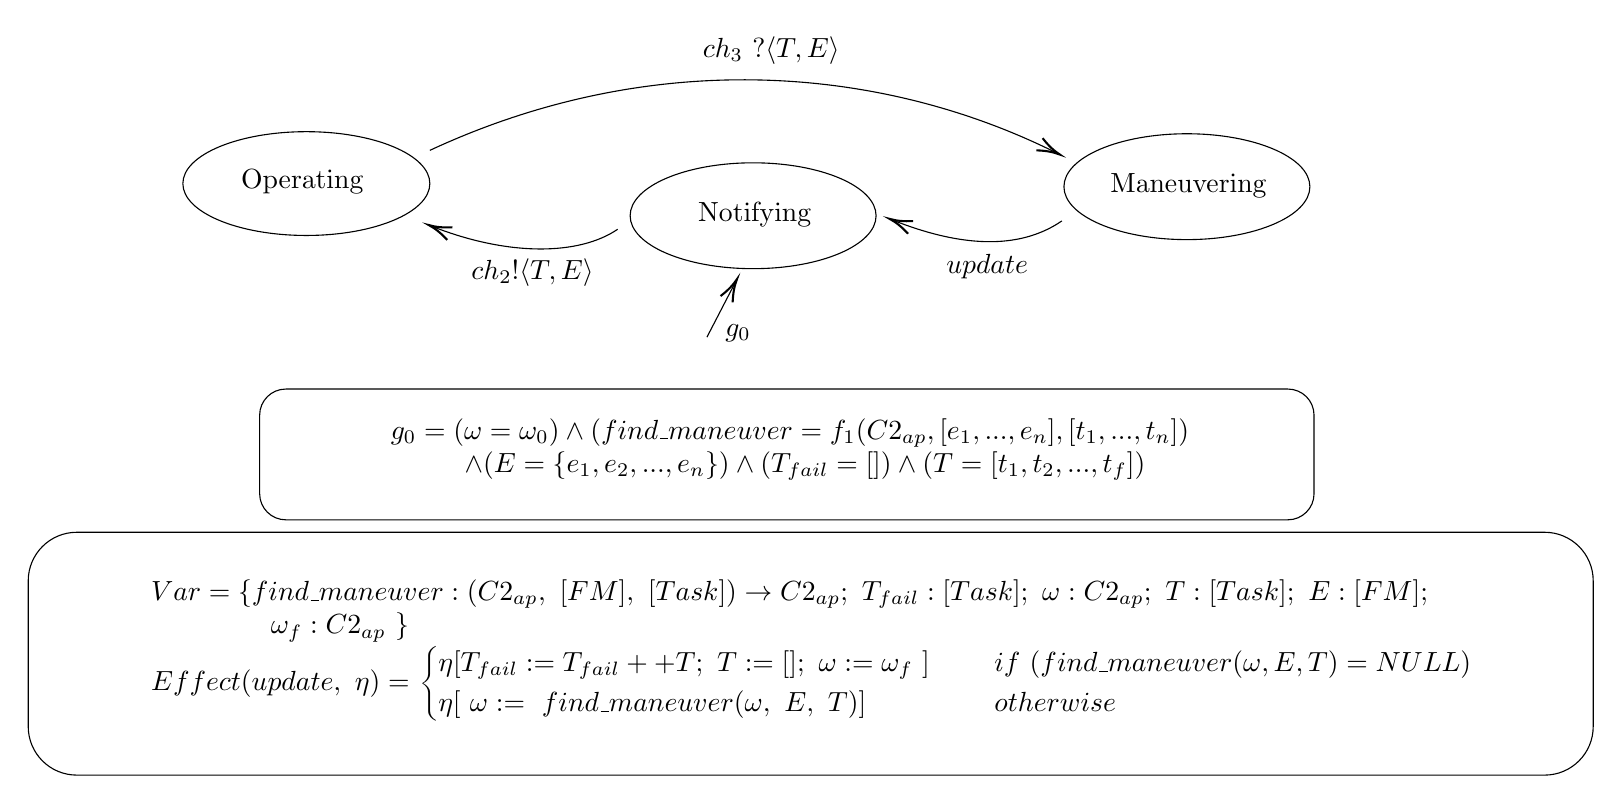
\begin{tikzpicture}[x=0.75pt,y=0.75pt,yscale=-1,xscale=1]
%uncomment if require: \path (0,370); %set diagram left start at 0, and has height of 370

%Curve Lines [id:da9480858267519683] 
\draw    (200.5,59) .. controls (307.46,9.25) and (417.89,17.91) .. (502.72,60.36) ;
\draw [shift={(504,61)}, rotate = 206.82999999999998] [color={rgb, 255:red, 0; green, 0; blue, 0 }  ][line width=0.75]    (10.93,-3.29) .. controls (6.95,-1.4) and (3.31,-0.3) .. (0,0) .. controls (3.31,0.3) and (6.95,1.4) .. (10.93,3.29)   ;
%Shape: Ellipse [id:dp6594609066072359] 
\draw   (81.5,75) .. controls (81.5,61.19) and (108.14,50) .. (141,50) .. controls (173.86,50) and (200.5,61.19) .. (200.5,75) .. controls (200.5,88.81) and (173.86,100) .. (141,100) .. controls (108.14,100) and (81.5,88.81) .. (81.5,75) -- cycle ;
%Shape: Ellipse [id:dp873836537729809] 
\draw   (506,76.5) .. controls (506,62.42) and (532.53,51) .. (565.25,51) .. controls (597.97,51) and (624.5,62.42) .. (624.5,76.5) .. controls (624.5,90.58) and (597.97,102) .. (565.25,102) .. controls (532.53,102) and (506,90.58) .. (506,76.5) -- cycle ;
%Straight Lines [id:da37650774099478246] 
\draw    (334,149) -- (347.58,122.78) ;
\draw [shift={(348.5,121)}, rotate = 477.38] [color={rgb, 255:red, 0; green, 0; blue, 0 }  ][line width=0.75]    (10.93,-3.29) .. controls (6.95,-1.4) and (3.31,-0.3) .. (0,0) .. controls (3.31,0.3) and (6.95,1.4) .. (10.93,3.29)   ;
%Rounded Rect [id:dp20897962983691354] 
\draw   (118.5,186.6) .. controls (118.5,179.64) and (124.14,174) .. (131.1,174) -- (613.9,174) .. controls (620.86,174) and (626.5,179.64) .. (626.5,186.6) -- (626.5,224.4) .. controls (626.5,231.36) and (620.86,237) .. (613.9,237) -- (131.1,237) .. controls (124.14,237) and (118.5,231.36) .. (118.5,224.4) -- cycle ;
%Rounded Rect [id:dp6489541210438411] 
\draw   (7,266.4) .. controls (7,253.48) and (17.48,243) .. (30.4,243) -- (737.6,243) .. controls (750.52,243) and (761,253.48) .. (761,266.4) -- (761,336.6) .. controls (761,349.52) and (750.52,360) .. (737.6,360) -- (30.4,360) .. controls (17.48,360) and (7,349.52) .. (7,336.6) -- cycle ;
%Shape: Ellipse [id:dp35747792046006877] 
\draw   (297,90.5) .. controls (297,76.42) and (323.53,65) .. (356.25,65) .. controls (388.97,65) and (415.5,76.42) .. (415.5,90.5) .. controls (415.5,104.58) and (388.97,116) .. (356.25,116) .. controls (323.53,116) and (297,104.58) .. (297,90.5) -- cycle ;
%Curve Lines [id:da035475864760055154] 
\draw    (424.21,92.88) .. controls (460.08,106.96) and (486.38,105.74) .. (505,93) ;
\draw [shift={(422,92)}, rotate = 22.07] [color={rgb, 255:red, 0; green, 0; blue, 0 }  ][line width=0.75]    (10.93,-3.29) .. controls (6.95,-1.4) and (3.31,-0.3) .. (0,0) .. controls (3.31,0.3) and (6.95,1.4) .. (10.93,3.29)   ;
%Curve Lines [id:da19760874620395663] 
\draw    (202.22,95.88) .. controls (238.39,109.99) and (272.38,109.74) .. (291,97) ;
\draw [shift={(200,95)}, rotate = 22.07] [color={rgb, 255:red, 0; green, 0; blue, 0 }  ][line width=0.75]    (10.93,-3.29) .. controls (6.95,-1.4) and (3.31,-0.3) .. (0,0) .. controls (3.31,0.3) and (6.95,1.4) .. (10.93,3.29)   ;

% Text Node
\draw (139,74) node   [align=left] {Operating};
% Text Node
\draw (566,76) node   [align=left] {Maneuvering};
% Text Node
\draw (365,11) node    {$ch_{3} \ ?\langle T,E\rangle $};
% Text Node
\draw (349,147) node    {$g_{0}$};
% Text Node
\draw (469,115) node    {$update$};
% Text Node
\draw (374,203) node    {$ \begin{array}{l}
g_{0} =( \omega =\omega _{0}) \land ( find\_maneuver=f_{1}( C2_{ap} ,[ e_{1} ,...,e_{n}] ,[ t_{1} ,...,t_{n}])\\
\ \ \ \ \ \ \ \ \land ( E=\{e_{1} ,e_{2} ,...,e_{n}\}) \land ( T_{fail} =[]) \land ( T=[ t_{1} ,t_{2} ,...,t_{f}])
\end{array}$};
% Text Node
\draw (385,300) node    {$ \begin{array}{l}
Var=\{find\_maneuver:( C2_{ap} ,\ [ FM] ,\ [ Task])\rightarrow C2_{ap} ;\ T_{fail} :[ Task] ;\ \omega :C2_{ap} ;\ T:[ Task] ;\ E:[ FM] ;\\
\ \ \ \ \ \ \ \ \ \ \ \ \ \omega _{f} :C2_{ap} \ \}\\
Effect( update,\ \eta ) =\begin{cases}
\eta [ T_{fail} :=T_{fail} ++T;\ T:=[] ;\ \omega :=\omega _{f} \ ] & \ \ \ \ if\ ( find\_maneuver( \omega ,E,T) =NULL)\\
\eta [ \ \omega :=\ find\_maneuver( \omega ,\ E,\ T)] & \ \ \ \ otherwise
\end{cases}
\end{array}$};
% Text Node
\draw (250,118) node    {$ch_{2} !\langle T,E\rangle $};
% Text Node
\draw (357,90) node   [align=left] {Notifying};

\end{tikzpicture}}
    \caption{C2 Approach Selector Role Program Graph}
    \label{fig:C2S}
\end{figure}

Finally, at the coarsest-grained level of coordination, C2A specifies a C2 approach change protocol (cf. Figure~\ref{fig:c2a_pg}). C2A starts operation by receiving mission tasks, member information, and initial C2 approach from the C2CS call ($g_0$ at location \textit{Notifying}). From this initial location, it goes to the location \textit{Operating} with the initial C2 approach $w_0$ and sends the set of tasks $T$ and the team $E$ through the synchronous channel $ch_2$. The C2A keeps in $Operating$ location up to eventually receive, from TA, the pair formed by the set of not allocated tasks and the team's members updated.Such information comes through the synchronous channel $ch_3$ and takes C2A to the location \textit{Maneuvering}.

The tasks received and the last information about the team are analysed with the action $update$. In case of the function \emph{find\_maneuver} be $NULL$, i.e., there is no C2 Approach to be operated in order to perform the tasks with the available team, we register those tasks as failed ($T_{fail}$) and we notify TA with an empty set of tasks. In such case, the C2A goes to the location \emph{Operating} passing through \emph{Notifying} and adopts a C2 Approach $w_f$ to be operated. This C2 Approach can be any one of the C2 Approach Space and it can guarantee more than one passing through the C2 Approaches. Otherwise, the  \emph{find\_maneuver} function returns a suitable C2 Approach to be operated following the diagonal in C2 Approach Space according to the maturity levels.
With C2 Approach defined, C2A sends mission's tasks and members' information to the TA over the synchronous channel $ch_2$, then moving to the location \emph{Operating}.


\newpage
\section{Design Implementation}
\label{sec:design}

Our proposed design, using program graphs and channel systems, models a group of entities coordinating to complete a common goal or objective while managing dynamic events. The team's members can be diverse, due to their different set of attributes and behaviours, according to their set of roles. Moreover, due to the heterogeneity of the group, each entity can react to various situations differently, in line with its information about the environment. Also, the communication topology among the team limits their interactions and can have a large impact on the overall system. With that in mind, and following related research~\cite{evaluating} our proposed design fits as an application of an agent-based model (ABM). 

To implement our application of an ABM, we used a framework on the Java platform, \textit{Repast Symphony}~\cite{repastDoc}. The aforementioned framework is commonly used for ABM simulations~\cite{repast} and it's capacity of simulating parallelism is mandatory in our domain. Finally, the underlying object-oriented paradigm is appropriate to encapsulate each role, i.e, program graph separately, simplifying adding or removing roles throughout the execution.

We chose our motivating example (Section \ref{sec:motivation}) as the theme of our implementation. Thus, each team member and its functionalities, i.e, onboard sensors and fuel capacity, is encapsulated in a \textit{Drone} class. Also, each role is represented by a \textit{Role} class, e.g, \textit{Executor}, \textit{TaskAllocator}, and \textit{C2ApproachSelector}. Moreover, auxiliary classes were made to add modularity and functionalities, such as providing the visual communication links between members and diversify input types to start the simulation. Based on the following research~\cite{swarmGap}, we used a token-based communication protocol to exchange information among the team (class \textit{Token}), whereas the communication channels, members specification, and task allocation information are being represented by \textit{Lists}. Figure \ref{fig:ClassDiagram} shows a class diagram of the implementation.

In every round of execution, i.e, in a single time unit (tick) of the simulation, all members execute its \textit{step} method. Additionally, each member performs the \textit{step} method of its roles, which follows the program graphs described in Section 3. For instance, the task allocator (Figure \ref{fig:TA}) role class first check information inside the channel $ch_1$ to receive feedback from the executors. Next, it executes a task allocation algorithm, using the current C2 approach provided by the received Token. If the allocation process is not successful, it informs the C2 approach selector role, adding this information to the channel $ch_3$.

Similarly, the main method of the C2 approach selector role's class (\textit{step}) implements its program graph (Figure \ref{fig:C2S}). First, it checks if the task allocator role sent information along the channel $ch_3$. If a maneuver was requested, it assesses a different C2 approach using some criteria, such as defined in the following research~\cite{france2014}. In case that a change is required, it finishes execution updating maneuver variables in the Token class, asking for the team's confirmation to switch to the new C2 approach.

The full implementation and auxiliary artifacts are available in a public repository\footnote{\gitRepository}.

\begin{figure}[ht]
  \centering
  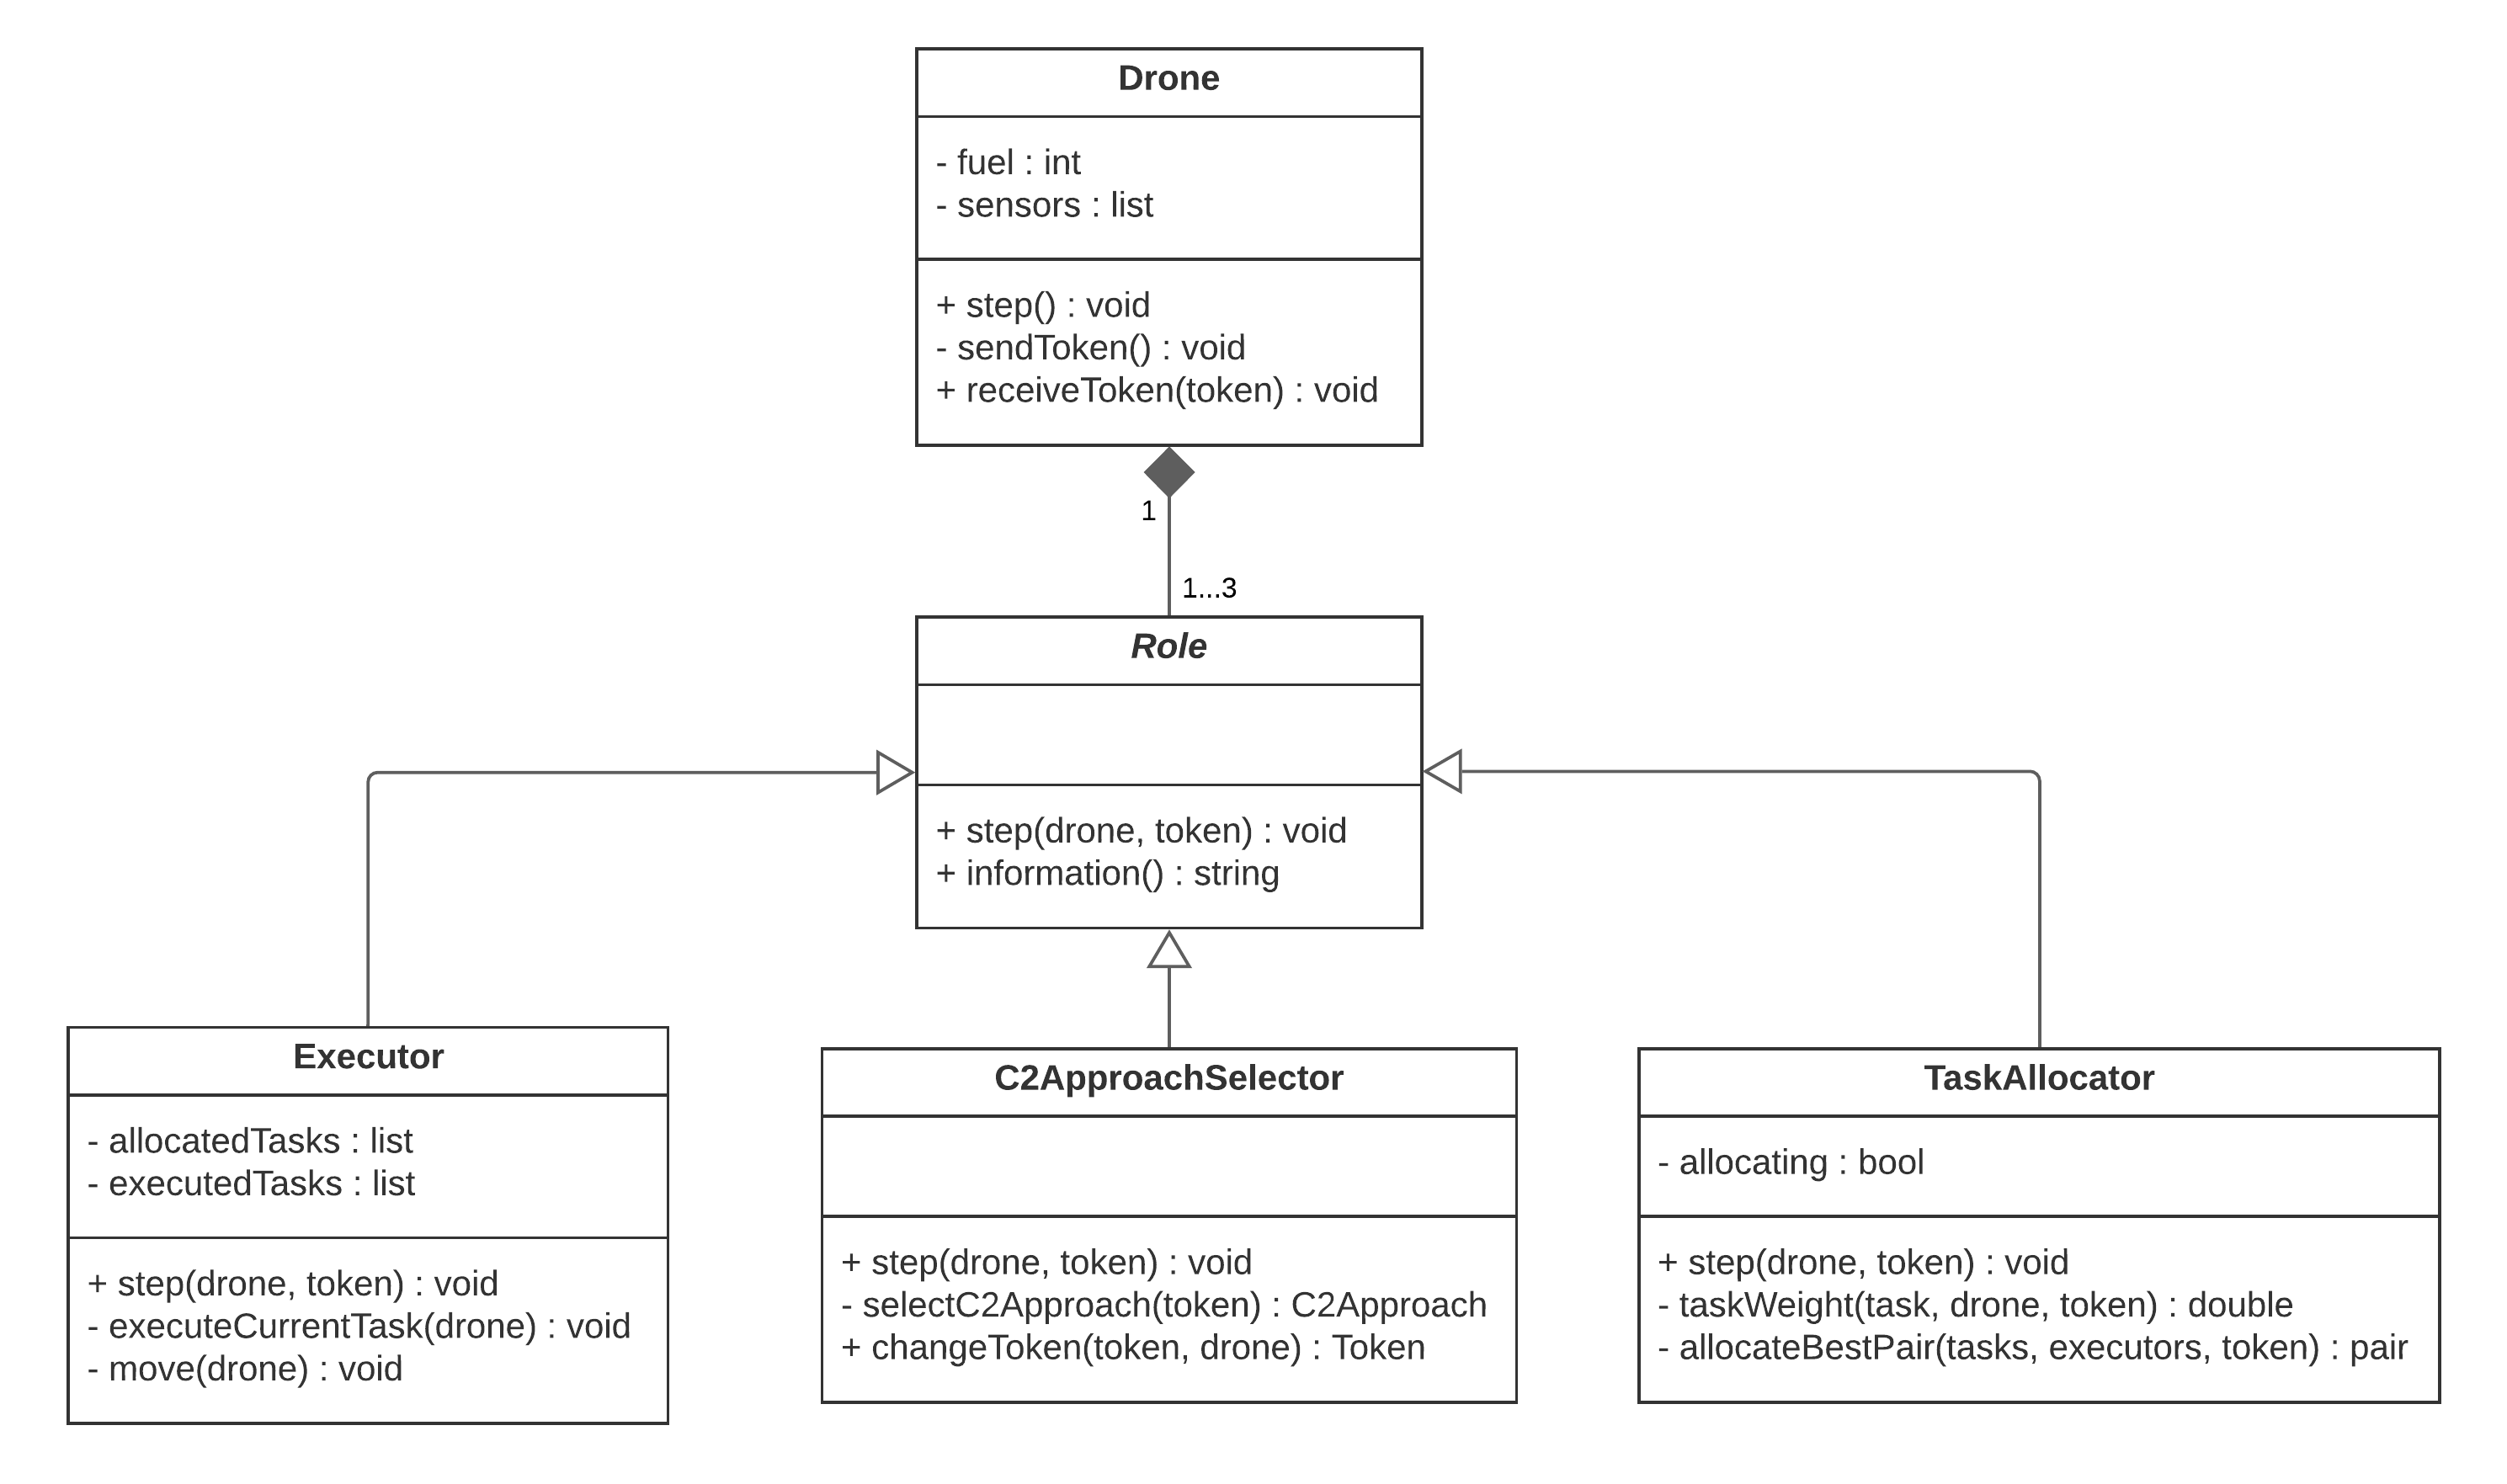
\includegraphics[width=0.9\linewidth]{figures/diagramaDeClasse.png}
  \captionof{figure}{Implementation's Class Diagram}
  \label{fig:ClassDiagram}
\end{figure}

% ROLE-BASED MODELING SECTION

% Also, because we separate a group of reusable functionalities encapsulated in different roles, our approach also applies principles from role-based modeling~\cite{roleOrientedModeling}.

% Finally, separating a group of reusable functionalities in different roles, i.e, in different program graphs, is an implementation design of role-based modeling~\cite{roleOrientedModeling, modelingAgentOrganizationsUsingRoles}.

% Roles are used to form different interfaces for agents in order to restrict the visibility of features~\cite{roleOrientedModeling}, such as internal attributes. Concerning their internal behaviour roles may capture goals and handle responsibilities~\cite{roleOrientedModeling} to execute tasks autonomously. Additionally, as demonstrated in Section \ref{subsec:PG}, roles can be dynamically attached to and retracted from an agent. This feature is especially important if a role shall migrate from one agent to another~\cite{roleOrientedModeling} in run time. For instance, when a maneuver occurs some agents may undergo a complete transformation in its roles, depending on the role of the C2 approach selector to decide which set of roles is more appropriate for each agent.

% A role class can be described in terms of its breath and dept~\cite{modelingAgentOrganizationsUsingRoles}. Breadth, or horizontal specialization, addresses the number and complexity of actions supported by a given role~\cite{modelingAgentOrganizationsUsingRoles}. Depth, or vertical specialization, relates to the degree of control an agent can have over its actions and the actions of other agents~\cite{modelingAgentOrganizationsUsingRoles}. Recalling Section \ref{sec:introduction}, horizontal specialization is more related to C2 Approach Agility, due to its nature of providing agility within the same C2 approach, adding resilience and flexibility in the current structure of execution. Similarly, vertical specialization relates to C2 Maneuver Agility. Dept relates to the task allocator and C2 approach selector roles, due to their level of influence over the remaining members while performing a maneuver or even which tasks they will execute.

\section{Evaluation}
\label{sec:evaluation}

To measure the obtained C2 system maneuver agility, we assessed the proposed model under different scenarios based on the definition of the capacity to deal with dynamic circumstances and changing its C2 approach according to some criteria. This assessment is performed through an \textit{in silico} experiment~\cite{simulation01} simulating our motivating example (Section \ref{sec:motivation}). Such a method provides a way to analyze different situations and it allows us to work with different scenarios that would otherwise be unfeasible to test given incurred cost and resources availability. The simulated environment considers that the circumstances can change during the mission execution, allowing to test the effectiveness of the C2 System under such conditions. Thus, our goal with the simulations is to answer the following research question:
 
\begin{center}
\fbox{\begin{minipage}{21em}
\textit{How much C2 maneuver agility does the system have?}
\end{minipage}}    
\end{center}

Next, we define the metrics applied in the evaluation to answer the proposed question and their corresponding descriptions:
\begin{itemize}
    \item Maneuvering (M1): Number of C2 Maneuvers performed by the members to accomplish the mission within a given timeout;
    \item Timeliness (M2): System time, in ticks, to accomplish the mission within a given timeout;
    \item Effectiveness (M3): Percentage of successful tasks completed by the executors.
\end{itemize}

Each scenario of the simulation executed considering two distinct methods of system response, i.e, A1 and A2. With A1 method, the system starts the execution with an initial context predefined and it performs a task allocation, i.e, distributing the mission received, and in face of context changes, e.g, member dropped, the system keeps running, but it does not perform any kind of adaptation to deal with new circumstances. In its turn, the A2 method applies the C2 computational design proposed in Section~\ref{sec:channelSystem} and whose implementation is described in Section~\ref{sec:design}. Ultimately, we compare the results obtained from each method, i.e, answer for the research question, to confirm the presence of increased level of C2 maneuver agility.

%%%%%%%%%%%%%%%%%%%%%%%%%%%%%%%%%%
% SUBSECTION 
%%%%%%%%%%%%%%%%%%%%%%%%%%%%%%%%%%
\subsection{Simulation Scenarios}
\label{sub:scenarios}

A simulation scenario is composed of an initial context and a sequence of events that provide dynamism. The initial context comprises the set $E$ of members operating an initial C2 Approach $\omega$, the mission $M$ composed of a set of tasks, and the environment. Each possible event, e.g, \textit{memberFailure}, \textit{sensorFailure}, and \textit{envChange}, represents an action that causes a member or environment changes in runtime. These actions are called during simulation to create a dynamic scenario, resembling realistic settings.

The environment represents all the conditions of the place where the members act, e.g, weather conditions, hazard, and communication restrictions, and it is modelled as the state of a specific kind of onboard sensor, e.g, a foggy day can turn a VGA sensor useless.

The scenarios were created with different sequences of actions (Table \ref{tab:scenarios}), i.e, context changes, combined with the same initial context, i.e., members, mission, environment and the initial C2 Approach. During simulation, all these changes occur within the timeout, i.e., mission time limit, but not equally distributed over time. The presented sequence is attended but the exact moment is aleatory.

\begin{table}[h]
\centenring
\fontsize{9}{9}
\selectfont
\caption{List of events(\textit{EC-envChange; SF-sensorFailure; MF-memberFailure}) that characterizes the context changes within the scenarios tested. The initial C2 Approach, the set of members $E$ and the mission $M$ remain unchanged.}
\label{tab:scenarios}
\begin{tabular}{|m{0.1\textwidth}|m{0.84\textwidth}|}
\hline
\rowcolor{lightgray}
 \textbf {Scenario} & \hfil  \textbf {Context Changes} \\
\hline
 \hfil 1 & EC $\rightarrow$ EC $\rightarrow$ EC $\rightarrow$ EC $\rightarrow$ EC\\
\hline 
 \hfil 2 & EC $\rightarrow$ EC $\rightarrow$ EC $\rightarrow$ EC $\rightarrow$ EC $\rightarrow$ EC $\rightarrow$ EC $\rightarrow$ EC $\rightarrow$ EC $\rightarrow$ EC $\rightarrow$ EC $\rightarrow$ EC $\rightarrow$ EC $\rightarrow$ EC $\rightarrow$ EC \\
\hline 
 \hfil 3 & 
EC $\rightarrow$ EC $\rightarrow$ EC $\rightarrow$ EC $\rightarrow$ EC $\rightarrow$ MF $\rightarrow$ EC $\rightarrow$ EC $\rightarrow$ EC $\rightarrow$ EC $\rightarrow$ EC $\rightarrow$ MF $\rightarrow$ EC $\rightarrow$ EC $\rightarrow$ EC $\rightarrow$ EC $\rightarrow$ EC $\rightarrow$ MF $\rightarrow$ EC $\rightarrow$ EC $\rightarrow$ EC $\rightarrow$ EC $\rightarrow$ EC  \\
\hline 
 \hfil 4 & EC $\rightarrow$ EC $\rightarrow$ EC $\rightarrow$ EC $\rightarrow$ EC $\rightarrow$ SF $\rightarrow$ EC $\rightarrow$ EC $\rightarrow$ EC $\rightarrow$ EC $\rightarrow$ EC $\rightarrow$ SF $\rightarrow$ EC $\rightarrow$ EC $\rightarrow$ EC $\rightarrow$ EC $\rightarrow$ EC $\rightarrow$ SF $\rightarrow$ EC $\rightarrow$ EC $\rightarrow$ EC $\rightarrow$ EC $\rightarrow$ EC  \\
\hline 
 \hfil 5 & EC $\rightarrow$ EC $\rightarrow$ EC $\rightarrow$ SF $\rightarrow$ EC $\rightarrow$ EC $\rightarrow$ EC $\rightarrow$ MF $\rightarrow$ EC $\rightarrow$ EC $\rightarrow$ EC $\rightarrow$ SF $\rightarrow$ EC $\rightarrow$ EC $\rightarrow$ EC $\rightarrow$ MF $\rightarrow$ EC $\rightarrow$ EC $\rightarrow$ EC $\rightarrow$ SF $\rightarrow$ EC $\rightarrow$ EC $\rightarrow$ EC $\rightarrow$ MF  \\
\hline 
 \hfil 6 & EC $\rightarrow$ SF $\rightarrow$ MF $\rightarrow$ EC $\rightarrow$ SF $\rightarrow$ EC $\rightarrow$ SF $\rightarrow$ EC $\rightarrow$ SF $\rightarrow$ MF $\rightarrow$ EC $\rightarrow$ SF $\rightarrow$ EC $\rightarrow$ SF $\rightarrow$ EC $\rightarrow$ SF \\
\hline 
 \hfil 7 & MF $\rightarrow$ SF $\rightarrow$ EC $\rightarrow$ EC $\rightarrow$ EC $\rightarrow$ EC $\rightarrow$ EC $\rightarrow$ EC $\rightarrow$ EC $\rightarrow$ EC $\rightarrow$ EC $\rightarrow$ EC $\rightarrow$ MF $\rightarrow$ SF $\rightarrow$ EC $\rightarrow$ EC $\rightarrow$ EC $\rightarrow$ EC $\rightarrow$ EC $\rightarrow$ MF $\rightarrow$ SF $\rightarrow$ EC $\rightarrow$ EC $\rightarrow$ EC $\rightarrow$ MF $\rightarrow$ SF $\rightarrow$ EC \\
 \hline
 \hfil 8 & MF $\rightarrow$ SF $\rightarrow$ EC $\rightarrow$ MF $\rightarrow$ SF $\rightarrow$ EC $\rightarrow$ MF $\rightarrow$ SF $\rightarrow$ EC $\rightarrow$ MF $\rightarrow$ SF $\rightarrow$ EC \\
 \hline
 \hfil 9 & SF $\rightarrow$ SF $\rightarrow$ SF $\rightarrow$ MF $\rightarrow$ SF $\rightarrow$ SF $\rightarrow$ SF $\rightarrow$ MF $\rightarrow$ SF $\rightarrow$ SF $\rightarrow$ SF $\rightarrow$ MF $\rightarrow$ SF $\rightarrow$ SF $\rightarrow$ SF \\
 \hline
 \hfil 10 & SF $\rightarrow$ EC $\rightarrow$ MF $\rightarrow$ SF $\rightarrow$ EC $\rightarrow$ MF $\rightarrow$ SF $\rightarrow$ EC $\rightarrow$ MF $\rightarrow$ SF $\rightarrow$ EC $\rightarrow$ MF $\rightarrow$ EC $\rightarrow$ EC $\rightarrow$ EC $\rightarrow$ EC $\rightarrow$ EC $\rightarrow$ EC $\rightarrow$ EC $\rightarrow$ EC $\rightarrow$ EC $\rightarrow$ EC \\
 \hline
\end{tabular}

\end{table}


The simulation operates a scenario with 5 possible types of tasks (0 to 4) and 5 types of sensors (A, B, C, D and E). The tasks and sensors onboard are randomly chosen before the running round. When the tasks allocation process starts, the algorithm applies a function that returns the quality $Q_{ij}$, obtained from a table, that correlates a sensor $i$ to the task $j$. When $Q_{ij}=0$ it means the sensor $i$ is not able to perform the task $j$.

A context change simulated by the system causes the quality reduction of a specific type of sensor, e.g., an environment change simulating a luminosity decreasing reduces in $50\%$ the quality of the sensor type 2 that represents a VGA camera. In case the sensor burns out, its quality comes to be zero and the task will be transmitted to another member to check its execution capacity. Furthermore, we can lose a member and, consequently, all its sensors onboard.

Context changes can generate situations such as the tasks reallocation is not enough to keep mission execution. In that case, the C2 System performs a C2 Approach change, i.e., maneuvering. The new C2 Approach operated can provide a higher awareness level, i.e., more information shared by the members with a new communication structure, and it can help the members perform reallocation based on the new data exchanged. The initial C2 Approach for all scenarios simulated is De-Conflicted, i.e, a ring communication structure. From this C2 Approach, the maneuver follows incrementally over a specific order of C2 approaches, based on the following research~\cite{france2014}, and going back to Conflicted after Edge. The Conflicted is the final C2 Approach adopted by the system before discarding the unfeasible tasks.

%%%%%%%%%%%%%%%%%%%%%%%%%%%%%%%%%%
% SUBSECTION 
%%%%%%%%%%%%%%%%%%%%%%%%%%%%%%%%%%
\subsection{Experimental Setup}
\label{sub:setup}

Figure \ref{fig:exp_setup} shows the experimental setup applied to assess C2 maneuver agility. A factorial experiment is performed with the treatments applied to the simulation scenario (Section~\ref{sub:scenarios}) and to the methods. Combinations of the factors are assessed with the metrics described in Section~\ref{ssec:definition}.

\begin{figure}[ht!]
    \centering
    \scalebox{.65}{

\tikzset{every picture/.style={line width=0.75pt}} %set default line width to 0.75pt        

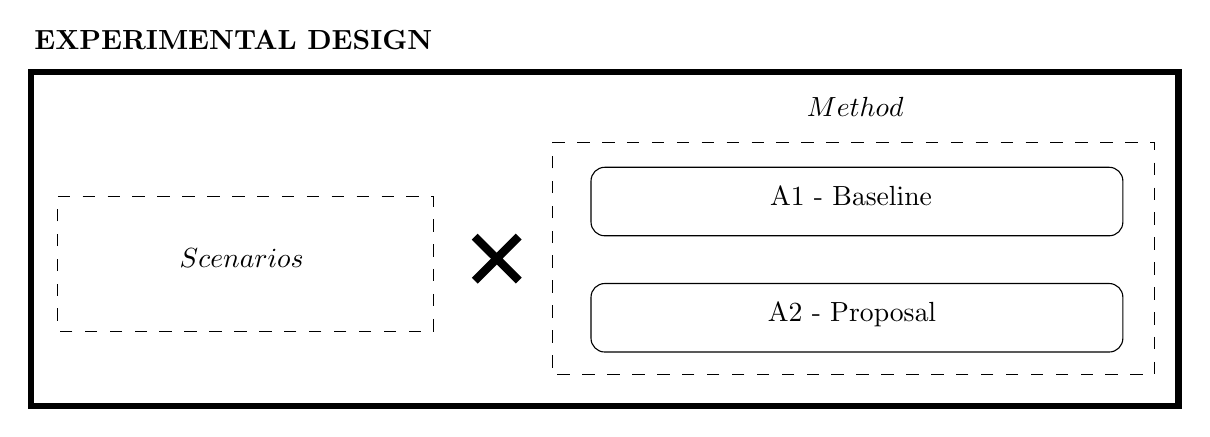
\begin{tikzpicture}[x=0.75pt,y=0.75pt,yscale=-1,xscale=1]
%uncomment if require: \path (0,201); %set diagram left start at 0, and has height of 201

%Rounded Rect [id:dp06575569211056953] 
\draw   (279.42,79.6) .. controls (279.42,75.95) and (282.37,73) .. (286.02,73) -- (529.06,73) .. controls (532.7,73) and (535.66,75.95) .. (535.66,79.6) -- (535.66,99.4) .. controls (535.66,103.05) and (532.7,106) .. (529.06,106) -- (286.02,106) .. controls (282.37,106) and (279.42,103.05) .. (279.42,99.4) -- cycle ;
%Shape: Rectangle [id:dp6932811140385843] 
\draw  [dash pattern={on 4.5pt off 4.5pt}] (22.5,87) -- (203.5,87) -- (203.5,152) -- (22.5,152) -- cycle ;
%Shape: Rectangle [id:dp9822494345299366] 
\draw  [dash pattern={on 4.5pt off 4.5pt}] (260.75,61) -- (551,61) -- (551,173) -- (260.75,173) -- cycle ;
%Shape: Rectangle [id:dp3952140034216508] 
\draw  [line width=2.25]  (9.5,27) -- (562.5,27) -- (562.5,188) -- (9.5,188) -- cycle ;
\draw  [line width=3]  (223.37,106.42) -- (244.63,127.58)(244.58,106.37) -- (223.42,127.63) ;
%Rounded Rect [id:dp9781270849297624] 
\draw   (279.42,135.6) .. controls (279.42,131.95) and (282.37,129) .. (286.02,129) -- (529.06,129) .. controls (532.7,129) and (535.66,131.95) .. (535.66,135.6) -- (535.66,155.4) .. controls (535.66,159.05) and (532.7,162) .. (529.06,162) -- (286.02,162) .. controls (282.37,162) and (279.42,159.05) .. (279.42,155.4) -- cycle ;

% Text Node
\draw (80,111) node [anchor=north west][inner sep=0.75pt]    {$Scenarios$};
% Text Node
\draw (382.17,38) node [anchor=north west][inner sep=0.75pt]    {$Method$};
% Text Node
\draw (10,6) node [anchor=north west][inner sep=0.75pt]   [align=left] {\textbf{EXPERIMENTAL DESIGN}};
% Text Node
\draw (364.41,81) node [anchor=north west][inner sep=0.75pt]   [align=left] {A1 - Baseline};
% Text Node
\draw (363.41,137) node [anchor=north west][inner sep=0.75pt]   [align=left] {A2 - Proposal};


\end{tikzpicture}}
    \caption{Experimental setup with the treatments performed by the simulator}
    \label{fig:exp_setup}
\end{figure}

The simulation uses a set of random variables to define some elements during execution, i.e, UAVs, and tasks position, and sensor that will be affected by the context event. For a consistent comparison between the methods A1 and A2, the same set of random variables is used by both methods during the same execution number.

Based on the following research~\cite{CochranW.G.1983}, the factorial experiment with the scenario and action method factors (Figure~\ref{fig:exp_setup}) was executed 500 times for all combinations of treatments. This sample size satisfies $95\%$ of confidence level~\cite{CochranW.G.1983}.

All scenarios created from the variables' values definition consider the same size of members' set $|E|=5$, the mission size $|M|=30$, and an initial C2 Approach $\omega_0 =$ De-Conflicted (Figure \ref{fig:scenario}). Finally, each simulation scenario has a deadline of 1000 ticks of execution time.

%%%%%%%%%%%%%%%%%%%%%%%%%%%%%%%%%%
% SUBSECTION 
%%%%%%%%%%%%%%%%%%%%%%%%%%%%%%%%%%
\subsection{Results and Analysis}

Table~\ref{table:results02} and Figures~\ref{fig:m1},~\ref{fig:m2}, and~\ref{fig:m3} show the results obtained by the simulation. Figure~\ref{fig:m1} shows the maneuvering (M1) metric results for all scenarios, not present in A1 method, with a more constant value due to the cost to perform a C2 Approach change.

\begin{figure}[ht]
\centering
\begin{minipage}{.5\textwidth}
    \centering
    \small
    \fontsize{7}{7}\selectfont
	\captionof{table}{Metrics results}
    \label{table:results02}
    \begin{tabular}{rrrr} \hline
		& \bf{M1}
        & \bf{M2}
		& \bf{M3} \\  \hline 
		
		& Mean(St.Dev.)  & Mean(St.Dev.) & Mean(St.Dev.)\\ [1ex]
		
		\multicolumn{3}{l}{\textbf{$\longrightarrow$ Scenario 1 }} \\
	% Scenario  1 
\bf{A1}  & 0.0 ($\pm$0.0)  & 890.0 ($\pm$66.8)  & 82.0 ($\pm$5.9)  \\
\bf{A2}  & 1.7 ($\pm$0.3)  & 945.5 ($\pm$33.1)  & 97.7 ($\pm$2.9)  \\ [1ex]
	
	\multicolumn{3}{l}{\textbf{$\longrightarrow$ Scenario 2 }} \\
% Scenario  2 
\bf{A1}  & 0.0 ($\pm$0.0)  & 866.5 ($\pm$72.3)  & 77.5 ($\pm$6.3) \\
\bf{A2}  & 2.6 ($\pm$0.6)  & 934.0 ($\pm$33.0)  & 95.2 ($\pm$4.2) \\ [1ex]
	
	\multicolumn{3}{l}{\textbf{$\longrightarrow$ Scenario 3 }} \\
% Scenario  3 
\bf{A1}  & 0.0 ($\pm$0.0)  & 782.1 ($\pm$78.3)  & 63.7 ($\pm$5.5) \\
\bf{A2}  & 2.8 ($\pm$0.3)  & 883.0 ($\pm$49.2)  & 69.1 ($\pm$4.5) \\ [1ex]
	
	\multicolumn{3}{l}{\textbf{$\longrightarrow$ Scenario 4 }} \\
% Scenario  4 
\bf{A1}  & 0.0 ($\pm$0.0)  & 799.1 ($\pm$77.0)  & 63.6 ($\pm$5.3) \\
\bf{A2}  & 3.0 ($\pm$0.1)  & 913.4 ($\pm$35.9)  & 84.5 ($\pm$5.1) \\ [1ex]
	
	\multicolumn{3}{l}{\textbf{$\longrightarrow$ Scenario 5 }} \\
% Scenario  5 
\bf{A1}  & 0.0 ($\pm$0.0)  & 733.7 ($\pm$75.5)  & 54.6 ($\pm$4.6)  \\
\bf{A2}  & 2.9 ($\pm$0.2)  & 887.7 ($\pm$48.4)  & 70.7 ($\pm$5.1) \\ [1ex]
	
	\multicolumn{3}{l}{\textbf{$\longrightarrow$ Scenario 6 }} \\
% Scenario  6 
\bf{A1}  & 0.0 ($\pm$0.0)  & 700.6 ($\pm$79.4)  & 42.0 ($\pm$4.5) \\
\bf{A2}  & 2.9 ($\pm$0.2)  & 910.5 ($\pm$59.3)  & 65.7 ($\pm$5.9) \\ [1ex]
	
	\multicolumn{3}{l}{\textbf{$\longrightarrow$ Scenario 7 }} \\
% Scenario  7 
\bf{A1}  & 0.0 ($\pm$0.0)  & 686.2 ($\pm$58.4)  & 41.1 ($\pm$3.5)  \\
\bf{A2}  & 2.8 ($\pm$0.3)  & 820.5 ($\pm$61.4)  & 60.1 ($\pm$5.6)  \\ [1ex]
	
	\multicolumn{3}{l}{\textbf{$\longrightarrow$ Scenario 8 }} \\
% Scenario  8 
\bf{A1}  & 0.0 ($\pm$0.0)  & 629.7 ($\pm$68.6)  & 36.3 ($\pm$3.8) \\
\bf{A2}  & 2.8 ($\pm$0.3)  & 785.1 ($\pm$58.3)  & 52.1 ($\pm$4.7) \\ [1ex]
	
	\multicolumn{3}{l}{\textbf{$\longrightarrow$ Scenario 9 }} \\
% Scenario  9 
\bf{A1}  & 0.0 ($\pm$0.0)  & 491.0 ($\pm$74.2)  & 26.4 ($\pm$3.7) \\
\bf{A2}  & 3.0 ($\pm$0.1)  & 743.2 ($\pm$66.1)  & 53.2 ($\pm$5.1) \\ [1ex]
	
	\multicolumn{3}{l}{\textbf{$\longrightarrow$ Scenario 10 }} \\
		
% Scenario  10 
\bf{A1}  & 0.0 ($\pm$0.0)  & 393.4 ($\pm$81.2)  & 24.3 ($\pm$2.6) \\
\bf{A2}  & 2.9 ($\pm$0.2)  & 650.7 ($\pm$114.8)  & 38.8 ($\pm$4.7) \\ [1ex]
		\hline
	\end{tabular}
\end{minipage}%
\begin{minipage}{.5\textwidth}
  \centering
  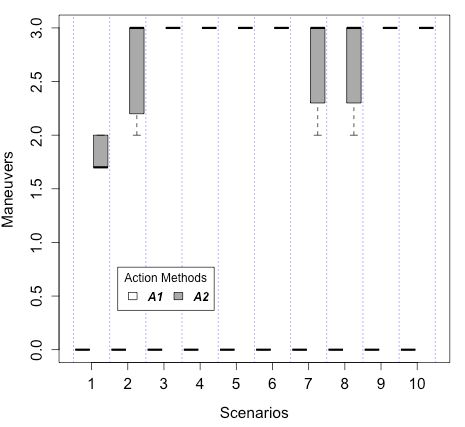
\includegraphics[width=0.95\linewidth]{figures/graphs/Boxplot_M2.png}
  \captionof{figure}{Total of maneuverings (M1)}
  \label{fig:m1}
\end{minipage}
\end{figure}

Notice in Figure~\ref{fig:m2} a significant difference between the system total time in the operation of the action methods, i.e, timeliness (M2). The choice of C2 Approach and how the C2 Approach space is explored, aspect only present in A2, come up against limitations of the entities' communication structure, as well as the cost for performing such maneuvers, i.e., time spent and entities' autonomy reduction. Although it took longer to complete the mission, the A2 method allowed the system to keep running for a longer time even in scenarios with more events that cause context changes compared with the A1 method. Figure~\ref{fig:m3} shows that the capacity of the C2 system to solve tasks, under the effect of changes in the context that alter its functioning, is more significant in the A2 method. 

Additionally, it is possible to identify, through the timeliness metric (M2), that more time consumed indicates a capacity to keep running under context perturbations and more resilience of the system to keep running even under such context changes. This characteristic is more present in A2 method due to the proposal tries to adapt itself to deal with these context changes and to keep running. 

\begin{figure}
\centering
\begin{minipage}{.5\textwidth}
  \centering
  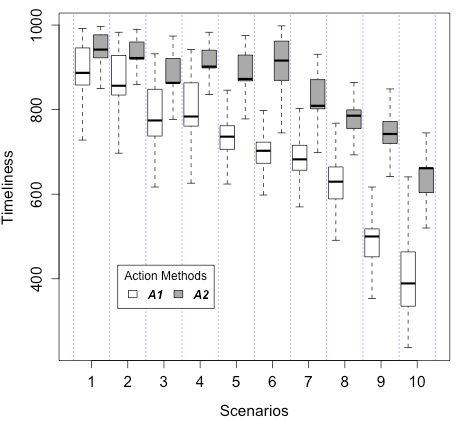
\includegraphics[width=0.95\linewidth]{figures/graphs/Boxplot_M3.png}
  \captionof{figure}{Total operation time (M2)}
  \label{fig:m2}
\end{minipage}%
\begin{minipage}{.5\textwidth}
  \centering
  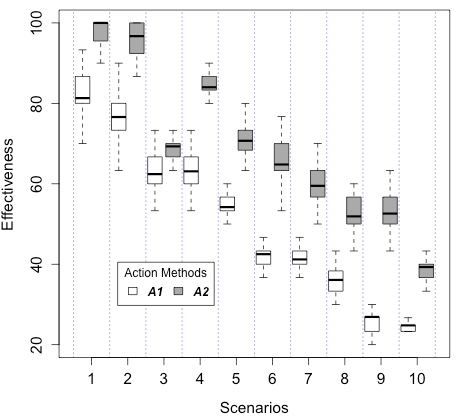
\includegraphics[width=0.95\linewidth]{figures/graphs/Boxplot_M5.png}
  \captionof{figure}{Completed tasks (M3)}
  \label{fig:m3}
\end{minipage}
\end{figure}


With a Shapiro-Wilk test~\citep{stat001} a \textit{p-value} less than 0.05 was obtained, thus indicating a non-normal distribution. Based on this, an Mann-Whitney U Test described in~\cite{stat002} was applied, i.e, Wilcoxon-test in R, to check differences among the samples of each action method applied, i.e, A1 and A2. According to the number and value of samples, the statistical analysis confirmed the difference between all results from A1 and A2 methods, collected in all scenarios tested.

In summary, the empirical findings indicate a better overall performance using the A2 method, despite its longer total execution time. Furthermore, it is possible to observe that the gain in the total amount of completed tasks is greater than the extra required time to finish the mission with the proposed A2 method. Such method enable the system to keep more time in action and allow a greater number of completed tasks. The capabilities embedded in the system result in a resilience increasing and enable the behavioral model the ability to cope with context changes and perturbations in dynamic scenarios.
 


\section{Conclusion}
\label{sec:conclusion}

Using the evaluation data (Section \ref{sec:evaluation}) as our base, we can conclude that providing more options to the agents, with different C2 approaches through maneuvers, increased performance in execution. This capability brings resilience and robustness to the overall system, due to the treatment of unexpected events.

Ultimately, the proposed design (Section \ref{sec:design}) has covered a lot of nuances in the simulation, e.g, sensor failure, drop of members. Sudden changes along execution were perceptible to the program graphs and were properly communicated to the right members using the channel systems, avoiding a significant drop in quality of the mission. Evidence provided by the simulation indicates that the presented design seems adequate to specify problems in the Command and Control domain.

%\section*{\refname}
%\bibliography{references}
\bibliography{references}
%qualifying

%\newpage
%\begin{appendices}
%
%\renewcommand\thefigure{\thesection.\arabic{figure}}
%\setcounter{figure}{0}
%
%\section{Probabilistic Models}
%\label{app:probabilistic-models}
%\input{content/appendix/models}
%
%\end{appendices}

\end{document}
